% !TeX program = xelatex
% ============================================================
% Document class
% ============================================================
\documentclass[11pt,a4paper]{report}

% ============================================================
% Language & Unicode (Greek FIRST)
% ============================================================
\usepackage{polyglossia}
\setdefaultlanguage{greek}
\setotherlanguage{english}

% ============================================================
% Fonts (XeLaTeX/LuaLaTeX) + Greek mappings for polyglossia
% ============================================================
\usepackage{fontspec}

\setmainfont{Linux Libertine O}
\setsansfont{Linux Biolinum O}
\setmonofont{Latin Modern Mono}

\newfontfamily\greekfont[
  Script=Greek,
  Language=Greek
]{Linux Libertine O}

\newfontfamily\greekfontsf[
  Script=Greek,
  Language=Greek
]{Linux Biolinum O}

\newfontfamily\greekfonttt[
  Script=Greek,
  Language=Greek
]{Latin Modern Mono}

% ============================================================
% Mathematics (unicode-math stack)
% ============================================================
\usepackage{amsmath}
\usepackage{mathtools}
\usepackage{unicode-math}

% Use a quiet, complete math font (fixes bold-shape warnings)
\setmathfont{Latin Modern Math}

% unicode-math safe bold vector and bold Greek parameters
\newcommand{\vect}[1]{\symbf{#1}}
\newcommand{\params}{\symbf{\theta}}
\newcommand{\dd}{\,\mathrm{d}}

\DeclareMathOperator{\Tr}{Tr}
\DeclareMathOperator{\diag}{diag}

% ============================================================
% Algorithms (pseudocode)
% ============================================================
\usepackage{algorithm}
\usepackage{algpseudocode}

% ============================================================
% Page layout
% ============================================================
\usepackage[
  left=25mm,
  right=25mm,
  top=25mm,
  bottom=30mm
]{geometry}

\setlength{\parindent}{0pt}
\setlength{\parskip}{6pt}

% ============================================================
% Figures & tables
% ============================================================
\usepackage{graphicx}
\usepackage{float}
\usepackage{caption}
\usepackage{subcaption}

\captionsetup{
  font=small,
  labelfont=bf,
  width=0.9\textwidth
}

\emergencystretch=2em


% ============================================================
% Colors (minimal)
% ============================================================
\usepackage{xcolor}
\definecolor{myblue}{RGB}{0,70,140}
\definecolor{defbg}{RGB}{246,250,255}
\definecolor{defborder}{RGB}{173,202,235}
\definecolor{thmbg}{RGB}{246,255,249}
\definecolor{thmborder}{RGB}{167,217,186}
\definecolor{toolbg}{RGB}{248,248,253}
\definecolor{toolborder}{RGB}{194,194,225}
\usepackage[most]{tcolorbox}
\newtcolorbox{definitionbox}[2]{
  enhanced,
  breakable,
  colback=defbg,
  colframe=defborder,
  boxrule=0.5pt,
  arc=1.6mm,
  left=2mm,
  right=2mm,
  top=1.2mm,
  bottom=1.2mm,
  title=\textbf{Ορισμός: #1}\hfill{\footnotesize\textcolor{myblue}{Πηγή: \cite{#2}}},
  fonttitle=\small\bfseries
}
\newtcolorbox{theorembox}[2]{
  enhanced,
  breakable,
  colback=thmbg,
  colframe=thmborder,
  boxrule=0.5pt,
  arc=1.6mm,
  left=2mm,
  right=2mm,
  top=1.2mm,
  bottom=1.2mm,
  title=\textbf{Θεώρημα: #1}\hfill{\footnotesize\textcolor{myblue}{Πηγή: \cite{#2}}},
  fonttitle=\small\bfseries
}
\newtcolorbox{toolbox}[2]{
  enhanced,
  breakable,
  colback=toolbg,
  colframe=toolborder,
  boxrule=0.5pt,
  arc=1.6mm,
  left=2mm,
  right=2mm,
  top=1.2mm,
  bottom=1.2mm,
  title=\textbf{Τεχνικός Ορισμός: #1}\hfill{\footnotesize\textcolor{myblue}{Πηγή: \cite{#2}}},
  fonttitle=\small\bfseries
}
\newtcolorbox{resultsbox}{
  enhanced,
  breakable,
  colback=white,
  colframe=thmborder!85!black,
  boxrule=0.8pt,
  arc=1.6mm,
  left=2mm,
  right=2mm,
  top=1.2mm,
  bottom=1.2mm,
  title=\textbf{Αποτελέσματα},
  coltitle=myblue,
  fonttitle=\small\bfseries
}
\newtcolorbox{importantbox}{
  enhanced,
  breakable,
  colback=white,
  colframe=toolborder!85!black,
  boxrule=0.8pt,
  arc=1.6mm,
  left=2mm,
  right=2mm,
  top=1.2mm,
  bottom=1.2mm,
  title=\textbf{Τεχνικό},
  coltitle=myblue,
  fonttitle=\small\bfseries
}
\newtcolorbox{guidebox}{
  enhanced,
  breakable,
  colback=white,
  colframe=defborder!85!black,
  boxrule=0.8pt,
  arc=1.6mm,
  left=2mm,
  right=2mm,
  top=1.2mm,
  bottom=1.2mm,
  title=\textbf{Οδηγίες},
  coltitle=myblue,
  fonttitle=\small\bfseries
}
\tcbset{
  appendixalgobox/.style={
    enhanced jigsaw,
    breakable,
    colback=toolbg,
    colframe=toolborder!85!black,
    boxrule=0.6pt,
    arc=1.4mm,
    left=1.5mm,
    right=1.5mm,
    top=1mm,
    bottom=1mm,
    before skip=0pt,
    after skip=0pt,
    before upper={\setlength{\parskip}{0pt}\setlength{\parindent}{0pt}\small}
  }
}

% ============================================================
% Hyperlinks
% ============================================================
\usepackage[
  colorlinks=true,
  linkcolor=myblue,
  citecolor=myblue,
  urlcolor=myblue
]{hyperref}

% ============================================================
% Bibliography
% ============================================================
\usepackage[numbers,sort&compress]{natbib}

% Optional (nice quotes in Greek text)
\usepackage{csquotes}

% ============================================================
% Section formatting
% ============================================================
\usepackage{titlesec}

\titleformat{\section}
  {\large\bfseries}
  {\thesection.}{0.6em}{}

\titleformat{\subsection}
  {\normalsize\bfseries}
  {\thesubsection.}{0.6em}{}

\titleformat{\subsubsection}
  {\normalsize\itshape}
  {\thesubsubsection.}{0.6em}{}

% ============================================================
% Title metadata
% ============================================================
\title{
\textbf{Ανάπτυξη Προσομοιωτή Μη Γραμμικών Δυναμικών Συστημάτων}\\
\large Εργαλείο για την μελέτη και την οπτικοποίηση της δυναμικής συμπεριφοράς τους.\\[4pt]
}

\author{
\Large Οδυσσέας Γκουντινάκος\\
\large Αριστοτέλειο Πανεπιστήμιο Θεσσαλονίκης\\
\large Επιβλέπων: Χρήστος Βόλος\\
}

\date{\small 10/03/2026}

% Build-path compatibility (compiling from project root or docs/thesis)
\graphicspath{{./}{docs/thesis/}}

% Resolve bibliography file regardless of working directory
\newcommand{\thesisbibfile}{refs}
\IfFileExists{refs.bib}{}{%
  \IfFileExists{docs/thesis/refs.bib}{\renewcommand{\thesisbibfile}{docs/thesis/refs}}{}%
}

% Lyapunov QR-study figures exported from the C++ pipeline
\IfFileExists{../../../nds_core_cpp/cpp_core/native/outputs_py/paper_figures/accuracy_stability_vs_qr.png}{%
  \newcommand{\lyastudyfigdir}{../../../nds_core_cpp/cpp_core/native/outputs_py/paper_figures}
}{%
  \newcommand{\lyastudyfigdir}{docs/thesis/../../../nds_core_cpp/cpp_core/native/outputs_py/paper_figures}
}

% ============================================================
% Document starts
% ============================================================
\begin{document}
% ============================================================
% Cover page (Εξώφυλλο)
% ============================================================
\begin{titlepage}
  \noindent
  \begin{minipage}[t]{0.22\textwidth}
    \vspace*{0pt}
    \raggedright
    \includegraphics[width=0.72\linewidth]{figures/auth_logo.png}
  \end{minipage}
  \begin{minipage}[t]{0.56\textwidth}
    \vspace*{0.65cm}
    \centering
    {\large Αριστοτέλειο Πανεπιστήμιο Θεσσαλονίκης\par}
    {\large Τμήμα Φυσικής\par}
    {\large Μεταπτυχιακό Πρόγραμμα Υπολογιστικής Φυσικής\par}
  \end{minipage}
  \begin{minipage}[t]{0.22\textwidth}
    \vspace*{0pt}
    \raggedleft
    \includegraphics[width=0.72\linewidth]{figures/comphys_logo.png}
  \end{minipage}

  \vspace*{0.9cm}
  \centering

  \vspace{1.2cm}

  {\LARGE\bfseries Ανάπτυξη Προσομοιωτή Μη Γραμμικών Δυναμικών Συστημάτων\par}
  \vspace{0.4cm}
  {\large Εργαλείο για την μελέτη και την οπτικοποίηση της δυναμικής συμπεριφοράς τους.\\[4pt]}


  \vfill

  {\Large\bfseries Οδυσσέας Γκουντινάκος\par}
  \vspace{0.2cm}
  {\large\bfseries Επιβλέπων: Χρήστος Βόλος\par}
  \vspace{0.25cm}
  {\normalsize \href{https://nlds-simulator.streamlit.app}{Non-linear Dynamical Systems Simulator}\par}
  \vspace{0.10cm}
  {\normalsize \href{https://github.com/OdyGoundi/nds-simulator}{Πλήρης Πηγαίος Κώδικας}\par}
  \vspace{0.25cm}
  {\large 10/03/2026\par}

\end{titlepage}

% ============================================================
% Abstract
% ============================================================
\begin{abstract}
\textbf{Περίληψη.}
Η εργασία παρουσιάζει τον σχεδιασμό, την υλοποίηση και την αξιολόγηση ενός επεκτάσιμου προσομοιωτή για μη γραμμικά δυναμικά συστήματα συνεχούς χρόνου, με στόχο την αξιόπιστη αριθμητική ανάλυση χαοτικών - συμβατικών και χαμιλτονιανών - συστημάτων. Ο προσομοιωτής επιλύει προβλήματα αρχικών τιμών σε $n$ διαστάσεις και παρέχει ενιαίο pipeline για χρονοσειρές, φασικά διαγράμματα, τομές Poincar\'e, διαγράμματα διακλάδωσης και εκτίμηση φάσματος εκθετών Lyapunov.

Στον αριθμητικό πυρήνα ενσωματώνονται μέθοδοι RK4, RK45, DOP853 και συμπλεκτικές μέθοδοι επίλυσης (Verlet, Forest-Ruth), ώστε η επιλογή μεθόδου να προσαρμόζεται στον τύπο της δυναμικής και στις απαιτήσεις διατήρησης γεωμετρικών ιδιοτήτων. Για τους εκθέτες Lyapunov υιοθετείται η κλασική προσέγγιση εξισώσεων μεταβολής με περιοδική ορθοκανονικοποίηση QR. Η μεθοδολογία υποστηρίζει τόσο αναλυτικό Ιακωβιανό όσο και αριθμητική προσέγγιση με κεντρικές διαφορές όταν δεν υπάρχει κλειστή μορφή. Έμφαση δίνεται στην επιλογή του διαστήματος επαναορθοκανονικοποίησης, επειδή επηρεάζει άμεσα τη σταθερότητα και τη σύγκλιση των εκτιμήσεων.

Η αρχιτεκτονική του λογισμικού διαχωρίζει καθαρά τη διεπαφή χρήστη από τον υπολογιστικό πυρήνα και υποστηρίζει πολλαπλά backends (Python, Numba, C++ επέκταση) για κλιμάκωση από διαδραστική εξερεύνηση έως απαιτητικά sweeps παραμέτρων. Η αξιολόγηση γίνεται σε αντιπροσωπευτικά συστήματα (Lorenz, R\"ossler, Duffing, H\'enon-Heiles), με συγκριτικά σενάρια ακρίβειας και επίδοσης και με έλεγχο αριθμητικών τεχνουργημάτων.

Κύρια συνεισφορά της εργασίας είναι η ενοποίηση θεωρίας, αλγορίθμων και οπτικοποίησης σε μία αναπαραγώγιμη ροή εργασίας που καθιστά διαφανή τη μετάβαση από την εξίσωση στο διαγνωστικό αποτέλεσμα. Το τελικό αποτέλεσμα αποτελεί πρακτικό πλαίσιο για εκπαιδευτική χρήση, διερευνητική μελέτη και περαιτέρω ερευνητική επέκταση.

\vspace{6pt}
\textbf{Abstract.}
This thesis presents the design, implementation, and evaluation of an extensible simulator for nonlinear continuous-time dynamical systems, targeting reliable numerical analysis in chaotic situations. The platform solves $n$-dimensional initial value problems and provides a unified workflow for time series, phase portraits, Poincar\'e sections, bifurcation diagrams, and Lyapunov spectrum estimation.

The numerical core combines RK4, RK45, DOP853, and symplectic integrators (Verlet and Forest-Ruth), allowing method selection based on dynamical behavior and long-time geometric fidelity requirements. Lyapunov exponents are computed through variational equations with periodic QR re-orthonormalization. Both analytic Jacobians and central finite-difference approximations are supported, enabling robust operation when closed-form derivatives are unavailable. Special emphasis is placed on QR reset period selection due to its direct impact on stability, convergence, and bias of finite-time estimates.

The software architecture cleanly separates user interface and computational engine, and supports multiple execution backends (Python, Numba, and a C++ extension) to balance interactivity and throughput for large parameter sweeps. Validation is carried out on representative benchmark systems (Lorenz, R\"ossler, Duffing, and H\'enon-Heiles), combining qualitative diagnostics with runtime and numerical-consistency checks.

The main contribution is an integrated, reproducible workflow that connects theory, algorithms, and visualization in a transparent path from model equations to interpretable diagnostics. The resulting framework is suitable for teaching, exploratory nonlinear analysis, and further research-oriented extensions.
\end{abstract}

\clearpage

\begin{center}
\fbox{\parbox[c][5.0cm][c]{0.88\textwidth}{\centering
Placeholder\\
Συνοπτικό σχήμα / visual abstract της εργασίας}}
\end{center}

\clearpage

% ============================================================
% Table of contents (Περιεχόμενα)
% ============================================================
\tableofcontents
\clearpage

% ============================================================
% Chapters
% ============================================================

\chapter{Θεωρητικό Υπόβαθρο και Υπολογιστική Μεθοδολογία}
\label{ch:theoretical-background-methodology}

\noindent\textbf{Σύνοψη Κεφαλαίου}.
\textenglish{}

\vspace{8pt}

\section{Πλαίσιο και Στόχοι του εργαλείου}
\label{sec:tool-context-goals}

Στην εργασία αυτή αναπτύχθηκε το εργαλείο \texttt{dynasim}, ένα πρόγραμμα με
γραφικό περιβάλλον που επιτρέπει τη μελέτη μη γραμμικών δυναμικών συστημάτων
συνεχούς χρόνου. Ο χρήστης μπορεί να ορίσει ένα σύστημα διαφορικών εξισώσεων
και να δει αριθμητικά τη συμπεριφορά του μέσω χρονοσειρών, διαγραμμάτων φάσης
και άλλων γραφικών εργαλείων.

Ένα σύστημα συνεχούς χρόνου περιγράφεται από την εξίσωση:

\begin{equation}
\dot{\mathbf{x}}=\mathbf{f}(\mathbf{x},t;\params),
\qquad
\mathbf{x}(t_0)=\mathbf{x}_0,
\end{equation}
όπου $\mathbf{x}\in\mathbb{R}^n$ και $\params$ διάνυσμα παραμέτρων.

Η παραπάνω σχέση εκφράζει το πώς αλλάζει η κατάσταση του συστήματος με τον
χρόνο. Στα απλά προβλήματα η λύση μπορεί να βρεθεί αναλυτικά. Στα περισσότερα
όμως μη γραμμικά συστήματα αυτό δεν είναι εφικτό, οπότε χρησιμοποιούμε
\textbf{αριθμητική λύση}: υπολογίζουμε δηλαδή προσεγγιστικές τιμές της λύσης
σε διακριτές χρονικές στιγμές.

Στόχος του εργαλείου είναι να βοηθήσει στη μελέτη αυτής της συμπεριφοράς,
ιδιαίτερα όταν το σύστημα γίνεται πολύπλοκο ή χαοτικό και δεν αρκεί η
αναλυτική μελέτη μόνο των εξισώσεων.

 \subsection{Μη Γραμμικά Δυναμικά Συστήματα}
\label{subsec:nonlinear-dynamical-systems}

Μη γραμμικό δυναμικό σύστημα ονομάζουμε ένα σύστημα του οποίου οι διαφορικές
εξισώσεις περιέχουν μη γραμμικούς όρους. Εξαιτίας αυτών των όρων, η
συμπεριφορά του συστήματος μπορεί να γίνει πολύ πιο πλούσια από ό,τι στα
γραμμικά συστήματα: μπορεί να εμφανιστούν περιοδικές τροχιές, πολύπλοκες
ταλαντώσεις ή και χαοτική συμπεριφορά.

\paragraph{Παράδειγμα 1 (Εκκρεμές).}
Θεωρούμε το ακόλουθο μοντέλο εκκρεμούς με τριβή:
\[
\dot{x}_1 = x_2,\qquad
\dot{x}_2 = -\frac{g}{l}\sin(x_1) - \frac{k}{ml}x_2.
\]
Εδώ $x_1$ είναι η γωνιακή θέση και $x_2$ η γωνιακή ταχύτητα. Το σύστημα είναι
μη γραμμικό επειδή εμφανίζεται ο όρος $\sin(x_1)$. Η παρουσία αυτού του όρου
είναι αρκετή για να κάνει τη μελέτη του συστήματος πιο δύσκολη και συνήθως
απαιτεί αριθμητική προσέγγιση.


\subsection{Περιεχόμενα του εργαλείου}
Το εργαλείο εστιάζει σε τρεις βασικές πλευρές της μελέτης ενός μη γραμμικού
συστήματος:
\begin{itemize}
\item \textbf{Απεικόνιση της τροχιάς στον χώρο φάσεων:} Με αυτόν τον τρόπο
βλέπουμε τη γεωμετρική μορφή της δυναμικής του συστήματος.
\item \textbf{Μελέτη της εξάρτησης από μια παράμετρο:} Εξετάζουμε πώς αλλάζει
η μακροχρόνια συμπεριφορά όταν μεταβάλλεται μια παράμετρος του συστήματος.
\item \textbf{Ποσοτική μέτρηση της ευαισθησίας στις αρχικές συνθήκες:}
Χρησιμοποιούμε τους εκθέτες Lyapunov για να εκτιμήσουμε αν η δυναμική είναι
περιοδική ή χαοτική.
\end{itemize}

Στις επόμενες ενότητες παρουσιάζονται με απλό τρόπο οι βασικές έννοιες και οι
αριθμητικές μέθοδοι που χρειάζονται για να παραχθούν αυτά τα αποτελέσματα.

\section{Αριθμητική Παραγωγή Φασικών Διαγραμμάτων}
\label{sec:numerical-phase-portraits}

\subsection{Από την ροή στην τροχιά}
\label{subsec:flow-to-trajectory}

Κάθε συνεχές δυναμικό σύστημα που περιγράφεται από την εξίσωση 
\begin{equation}
\dot{\mathbf{x}} = \mathbf{f}(\mathbf{x},t), \qquad \mathbf{x}(t_0)=\mathbf{x}_0,
\end{equation}
περιγράφεται από ένα \textbf{σύστημα διαφορικών εξισώσεων}. Αν γνωρίζουμε την αρχική
κατάσταση $\mathbf{x}_0$ στη χρονική στιγμή $t_0$, τότε ζητούμε να βρούμε τη
λύση $\mathbf{x}(t)$ για μεταγενέστερους χρόνους. Η λύση αυτή ονομάζεται
\textbf{τροχιά} του συστήματος.

\begin{definitionbox}{Διάγραμμα Φάσης}{maaita_meletlidou_kallipos}
  Σε ένα αυτόνομο δυναμικό σύστημα, οι δυναμικές μεταβλητές
  $x_1(t), x_2(t), \dots, x_n(t)$ διαμορφώνουν έναν $n$-διάστατο χώρο, ο οποίος
  ονομάζεται χώρος φάσεων (\foreignlanguage{english}{phase space}). Για κάθε χρονική
  στιγμή, η λύση $\bigl(x_1(t), x_2(t), \dots, x_n(t)\bigr)$ καθορίζει ένα σημείο
  του χώρου φάσεων. Το σύνολο αυτών των σημείων σχηματίζει μία καμπύλη στον χώρο
  φάσεων, η οποία ονομάζεται φασική τροχιά ή απλά τροχιά. Το σύνολο όλων των
  φασικών τροχιών ονομάζεται διάγραμμα φάσης.
\end{definitionbox}

Το διάγραμμα φάσης είναι ένα από τα πιο βασικά εργαλεία οπτικοποίησης. Δεν μας
δείχνει απλώς τιμές ως προς τον χρόνο, αλλά τη γεωμετρία της δυναμικής του
συστήματος. Έτσι μπορούμε να ξεχωρίσουμε αν η τροχιά τείνει σε ισορροπία,
αν επαναλαμβάνεται περιοδικά ή αν γίνεται πιο σύνθετη.

Στο επόμενο σχήμα φαίνονται δύο χαρακτηριστικά παραδείγματα φασικών
πορτραίτων, ένα για το σύστημα Lorenz και ένα για το σύστημα H\'enon-Heiles.

\begin{figure}[H]
  \centering
  \begin{subfigure}{0.49\textwidth}
    \centering
    
\includegraphics[width=\textwidth]{lorenz_3d_phase_space.png}
    \caption{\textbf{Lorenz:} $\sigma=10$, $\rho=28$, $\beta=\tfrac{8}{3}$, $y(0)=(1,1,1)$.}
    \label{fig:lorenz-phase-portrait}
  \end{subfigure}
  \hfill
  \begin{subfigure}{0.49\textwidth}
    \centering
    \includegraphics[width=\textwidth]{henon-heiles_phase_space.png}
    \caption{\textbf{H\'enon-Heiles:} $\lambda=2.79$, $y(0)=(0.1,0,0,0.1)$.}
    \label{fig:henon-heiles-phase-portrait}
  \end{subfigure}
  \caption{Παραδείγματα φασικών πορτρέτων για δύο διαφορετικά δυναμικά συστήματα.}
  \label{fig:phase-portraits-examples}
\end{figure}

Στην πράξη, η τροχιά δεν υπολογίζεται ως ακριβής συνεχής καμπύλη αλλά με
\textbf{αριθμητική λύση}. Αυτό σημαίνει ότι υπολογίζουμε προσεγγιστικές τιμές
της λύσης σε διακριτές χρονικές στιγμές, π.χ.\ $t_0,t_1,t_2,\dots$.

Η αριθμητική παραγωγή φασικών διαγραμμάτων ανάγεται στον αξιόπιστο
υπολογισμό της τροχιάς
\begin{equation}
\mathbf{x}_k \approx \mathbf{x}(t_k),
\qquad t_k = t_0 + k\Delta t,
\end{equation}
και στη συνέχεια στην απεικόνιση προβολών όπως $(x_i(t_k), x_j(t_k))$ ή
$(x_i, x_j, x_k)$.

Συνεπώς, για να παραχθεί ένα διάγραμμα φάσης χρειάζονται δύο βήματα:
πρώτα ο υπολογισμός της αριθμητικής λύσης και έπειτα η γραφική απεικόνιση της
τροχιάς σε δύο ή τρεις διαστάσεις.

\subsection{IVP (initial value problem) επιλύσεις: προσαρμοστικό βήμα, σταθερό βήμα και ειδικες συμπλεκτικές μέθοδοι.}
\label{subsec:ivp-solvers}

Το πρόβλημα εύρεσης της λύσης ενός συστήματος όταν είναι γνωστή η αρχική
κατάσταση ονομάζεται \textbf{πρόβλημα αρχικών τιμών}
(\foreignlanguage{english}{initial value problem}, IVP). Για την αριθμητική
του επίλυση, το εργαλείο υποστηρίζει τρεις βασικές κατηγορίες μεθόδων:

\begin{itemize}
\item \textbf{Μέθοδοι σταθερού βήματος:} το βήμα χρόνου παραμένει σταθερό σε
όλη τη διάρκεια της ολοκλήρωσης.
\item \textbf{Μέθοδοι προσαρμοστικού βήματος:} το βήμα χρόνου αλλάζει
αυτόματα ανάλογα με τη δυσκολία του προβλήματος.
\item \textbf{Συμπλεκτικές μέθοδοι:} χρησιμοποιούνται κυρίως σε
Χαμιλτονιανά συστήματα, όπου θέλουμε καλύτερη συμπεριφορά σε μεγάλους χρόνους.
\end{itemize}

\subsection{Runge – Kutta 4ης Τάξης σταθερού βήματος (RK4 fixed step)}
\label{subsec:rk4-fixed-step}

Μία βασική επιλογή είναι και ο κλασικός RK4 σταθερού βήματος. Στην περίπτωση
αυτή ο χρήστης επιλέγει εξαρχής το βήμα
$\Delta t$ και το ίδιο βήμα χρησιμοποιείται σε όλη την ολοκλήρωση.

Η μέθοδος αυτή είναι χρήσιμη όταν θέλουμε σταθερή δειγματοληψία στον χρόνο,
πιο απλή σύγκριση αποτελεσμάτων ή καλύτερο έλεγχο του πλέγματος χρόνου.
Μειονέκτημά της είναι ότι η ποιότητα του αποτελέσματος εξαρτάται άμεσα από το
πόσο κατάλληλο είναι το επιλεγμένο βήμα. Ο αναλυτικός τύπος του RK4 δίνεται στο
Παράρτημα~\ref{app:rk4-formula}.

\subsection{Αριθμητική Ολοκλήρωση με Προσαρμοστικό Βήμα}
\label{subsec:adaptive-step-integration}

Στις μεθόδους προσαρμοστικού βήματος, το πρόγραμμα δεν χρησιμοποιεί πάντα το
ίδιο $\Delta t$. Όταν η λύση αλλάζει γρήγορα, το βήμα μικραίνει ώστε ο
υπολογισμός να γίνει πιο αξιόπιστος. Όταν η λύση μεταβάλλεται πιο ομαλά, το
βήμα μπορεί να μεγαλώσει ώστε να μειωθεί ο υπολογιστικός χρόνος.

Στην κατηγορία αυτή ανήκουν οι μέθοδοι RK45 και DOP853. Και οι δύο είναι
γενικής χρήσης και κατάλληλες για πολλά μη γραμμικά συστήματα, ειδικά όταν
θέλουμε καλή ακρίβεια χωρίς να επιλέγουμε χειροκίνητα κάθε φορά το βήμα
χρόνου. Οι βασικές εξισώσεις των δύο μεθόδων δίνονται στο
Παράρτημα~\ref{app:adaptive-rk-formulas}.

\subsection{Συμμετρικές μέθοδοι για Χαμιλτονιανά συστήματα}
\label{subsec:symplectic-integrators-hamiltonian}

Σε Χαμιλτονιανά συστήματα, έχει
ιδιαίτερη σημασία η σωστή ενεργειακή συμπεριφορά - να διατηρείται - για μεγάλο χρόνο 
αριθμητικού υπολογισμού.
Γι' αυτό χρησιμοποιούνται συμπλεκτικές μέθοδοι, όπως οι Verlet και
Forest-Ruth, οι οποίες είναι σχεδιασμένες ώστε να αποδίδουν πιο πιστά τη
μακροχρόνια δυναμική τέτοιων συστημάτων
\cite{hairer_lubich_wanner,lubich_symplectic}.

Αντίθετα, μια γενική μέθοδος όπως η Runge-Kutta μπορεί να δίνει πολύ καλή
τοπική προσέγγιση αλλά σε μεγάλους χρόνους να παρουσιάζει τεχνητή ολίσθηση
στην ενέργεια.

Για να φανεί αυτή η διαφορά, χρησιμοποιήθηκε ως παράδειγμα το χαμιλτονιανό
σύστημα H\'enon-Heiles. Συγκρίθηκε η μέθοδος Forest-Ruth με την RK45, με ίδιες
αρχικές συνθήκες και ίδιες βασικές ρυθμίσεις ολοκλήρωσης. Οι εξισώσεις των
Verlet και Forest-Ruth δίνονται στο Παράρτημα~\ref{app:symplectic-formulas}.
\begin{resultsbox}
Το βασικό συμπέρασμα είναι ότι η Forest-Ruth διατηρεί την ενέργεια πρακτικά
σταθερή, ενώ η RK45 εμφανίζει αισθητή ολίσθηση. Αυτό δείχνει γιατί η επιλογή
μεθόδου ολοκλήρωσης δεν είναι μόνο θέμα ακρίβειας, αλλά και θέμα σωστής
ποιοτικής περιγραφής της φυσικής του προβλήματος.
\end{resultsbox}

\begin{table}[H]
  \centering
  \caption{Σύνοψη για την φαινομενική ολίσθηση στις τιμές της ενέργειας στο H\'enon-Heiles: Forest-Ruth έναντι RK45.}
  \label{tab:hh-energy-drift}
  \begin{tabular}{lccc}
    \hline
    Μέθοδος & $\max_t |\Delta H(t)|$ & RMS$(\Delta H)$ & $|\Delta H(t_{\mathrm{end}})|$ \\
    \hline
    Forest-Ruth (symplectic) & $4.121221\times10^{-11}$ & $2.545199\times10^{-11}$ & $3.200719\times10^{-11}$ \\
    RK45 (μη-symplectic) & $8.612698\times10^{-3}$ & $5.270482\times10^{-3}$ & $8.582167\times10^{-3}$ \\
    \hline
  \end{tabular}
\end{table}

Ο Πίνακας~\ref{tab:hh-energy-drift} περιγράφει τη διαφορά των δύο μεθόδων ως
προς την ενέργεια. Συμπληρωματικά, για να μετρήσουμε πόσο απέχουν συνολικά οι
δύο αριθμητικές λύσεις στον χώρο κατάστασης, χρησιμοποιούμε τη \textbf{νόρμα
απόκλισης}
\begin{equation}
\|\Delta \mathbf{y}(t)\|_2=
\|\mathbf{y}_{\mathrm{sym}}(t)-\mathbf{y}_{\mathrm{RK45}}(t)\|_2.
\end{equation}
Η ποσότητα αυτή είναι η ευκλείδεια απόσταση των δύο λύσεων τη χρονική στιγμή
$t$. Μικρή τιμή σημαίνει ότι οι δύο λύσεις είναι κοντά, ενώ μεγάλη τιμή
σημαίνει ότι έχουν απομακρυνθεί αισθητά.

Ακολουθεί η ενεργειακή σύγκριση Forest-Ruth και RK45 στο Henon-Heiles, τόσο για την τιμή της ενέργειας όσο και για την φαινομενική ολίσθησή της (drift).

\begin{figure}[H]
  \centering
  \begin{subfigure}{0.49\textwidth}
    \centering
    \includegraphics[width=\textwidth]{energy_for_hamiltonians/henon_heiles_hamiltonian_over_time.png}
    \caption{$H(t)$}
    \label{fig:hh-h-of-t}
  \end{subfigure}
  \hfill
  \begin{subfigure}{0.49\textwidth}
    \centering
    \includegraphics[width=\textwidth]{energy_for_hamiltonians/henon_heiles_energy_drift_over_time.png}
    \caption{$\Delta H(t)=H(t)-H(0)$}
    \label{fig:hh-dh-of-t}
  \end{subfigure}
  \caption{H\'enon-Heiles: ενεργειακή σύγκριση Forest-Ruth (μαύρο) και RK45 (magenta). Ο RK45 παρουσιάζει συστηματική ολίσθηση (drift), ενώ η συμπλεκτική μέθοδος (symplectic solver) διατηρεί την ενέργεια πρακτικά σταθερή.}
  \label{fig:hh-energy-comparison}
\end{figure}

Στο επόμενο σχήμα φαίνεται η χρονική εξέλιξη της νόρμας απόκλισης μεταξύ symplectic και RK45 λύσης στο Henon-Heiles.
Η ποσότητα αυτή εκφράζει την απόσταση των δύο λύσεων στον χώρο κατάστασης $(q_1,q_2,p_1,p_2)$ σε κάθε χρονική στιγμή.

\begin{figure}[H]
  \centering
  \includegraphics[width=0.78\textwidth]{energy_for_hamiltonians/henon_heiles_state_deviation_norm.png}
  \caption{Νόρμα απόκλισης κατάστασης $\|\mathbf{y}_{\mathrm{sym}}(t)-\mathbf{y}_{\mathrm{RK45}}(t)\|_2$ στο H\'enon-Heiles.}
  \label{fig:hh-state-deviation}
\end{figure}

\section{Αριθμητικός υπολογισμός διαγραμμάτων διακλάδωσης}
\label{sec:bifurcation-diagrams}

\subsection{Έννοια διαγράμματος διακλάδωσης}
\label{subsec:bifurcation-diagram-meaning}

\begin{definitionbox}{Διακλάδωση και διάγραμμα διακλάδωσης}{strogatz_nonlinear,guckenheimer_holmes,kuznetsov_bifurcation}
Ως \textbf{διακλάδωση} ορίζεται η ποιοτική μεταβολή της μακροχρόνιας
συμπεριφοράς ενός συστήματος όταν μια παράμετρος $\mu$ περάσει μια κρίσιμη
τιμή. Ένα \textbf{διάγραμμα διακλάδωσης} δείχνει πώς αλλάζει αυτή η
συμπεριφορά καθώς μεταβάλλεται η παράμετρος.
\end{definitionbox}

Στην πράξη, για κάθε τιμή της παραμέτρου $\mu$, το σύστημα ολοκληρώνεται
αριθμητικά και πρώτα απορρίπτεται το αρχικό μεταβατικό μέρος της τροχιάς.
Στη συνέχεια κρατούνται χαρακτηριστικά σημεία της τροχιάς, ώστε
το διάγραμμα να περιγράφει την ασυμπτωτική συμπεριφορά του συστήματος \cite{strogatz_nonlinear,guckenheimer_holmes}.

Η ερμηνεία του διαγράμματος γίνεται από την κατανομή των σημείων για κάθε
τιμή της $\mu$. Αν εμφανίζονται λίγα διακριτά σημεία, η κίνηση είναι συνήθως
περιοδική. Αν εμφανίζεται συνεχής ζώνη ή πυκνό νέφος σημείων, η συμπεριφορά
είναι πιο σύνθετη και μπορεί να είναι χαοτική. Με αυτόν τον τρόπο γίνονται
ορατές μεταβάσεις όπως ο πολλαπλασιασμός περιόδου και η μετάβαση προς το
χάος \cite{ott_chaos,kuznetsov_bifurcation}.

\subsection{Στροβοσκοπική απεικόνιση, χάρτης Poincar\'e και επιλογή χαρακτηριστικών σημείων}
\label{subsec:poincare-and-sampling}

\begin{definitionbox}{Στροβοσκοπική ακολουθία και χάρτης Poincaré}{koy_poincare_map_2016,guckenheimer_holmes,ott_chaos}
Σε ένα περιοδικά εξαναγκαζόμενο σύστημα μπορούμε να παρατηρούμε την τροχιά
ανά μία περίοδο $T$. Τα σημεία
\begin{equation}
\Pi=\{\mathbf{x}(t_0+kT)\}_{k\ge 0}
\end{equation}
σχηματίζουν τη \textbf{στροβοσκοπική ακολουθία}. Ο κανόνας που στέλνει κάθε
σημείο στο επόμενο λέγεται \textbf{χάρτης Poincaré}.
\end{definitionbox}

Η βασική ιδέα είναι ότι δεν χρειάζεται πάντα να μελετάμε ολόκληρη τη συνεχή
τροχιά. Συχνά αρκεί να κρατήσουμε ένα διακριτό σύνολο χαρακτηριστικών σημείων.
Έτσι η εικόνα γίνεται πιο απλή και είναι πιο εύκολο να ξεχωρίσουμε αν η
συμπεριφορά είναι περιοδική ή χαοτική \cite{koy_poincare_map_2016,ott_chaos}.

Στα περιοδικά εξαναγκαζόμενα συστήματα, αυτά τα σημεία παίρνονται συνήθως ανά
μία περίοδο. Στα αυτόνομα συστήματα, όπως το Lorenz, η ίδια ιδέα εφαρμόζεται
με μια κατάλληλη επιφάνεια $\Sigma$, και τότε κρατάμε τις διαδοχικές τομές της
τροχιάς με αυτήν, με συγκεκριμένη φορά διέλευσης \cite{guckenheimer_holmes,ott_chaos}.

Το παρακάτω σχήμα δείχνει ένα χαρακτηριστικό παράδειγμα για την εξίσωση
Duffing, όπου η στροβοσκοπική δειγματοληψία οδηγεί σε αποτύπωση του παράξενου
ελκυστή πάνω στην τομή Poincaré.

\begin{figure}[H]
  \centering
  \begin{subfigure}{0.49\textwidth}
    \centering
    \includegraphics[width=\textwidth]{strovo_poi_map_duff.png}
    \caption{Από την εφαρμογή dynasim.}
    \label{fig:stroboscopic-poincare-map-duff-dynasim}
  \end{subfigure}
  \hfill
  \begin{subfigure}{0.49\textwidth}
    \centering
    \includegraphics[width=\textwidth]{strovo_poi_map_duff_melet.png}
    \caption{Από το βιβλίο των Βουγιατζή και Μελετλίδου \cite{koy_poincare_map_2016}.}
    \label{fig:stroboscopic-poincare-map-duff-book}
  \end{subfigure}
  \caption{Αποτύπωση του παράξενου ελκυστή της εξίσωσης Duffing για $d=1/3$, $f_0=0.3$ και $x_0=y_0=0$ μέσω τομής στην επιφάνεια Poincaré. Αριστερά φαίνεται το αποτέλεσμα από την εφαρμογή dynasim και δεξιά η αντίστοιχη αποτύπωση από το βιβλίο των Βουγιατζή και Μελετλίδου \cite{koy_poincare_map_2016}.}
  \label{fig:stroboscopic-poincare-map}
\end{figure}

Για να κατασκευαστεί ένα διάγραμμα διακλάδωσης, συνήθως δεν κρατάμε ολόκληρο
το σημείο της τομής αλλά μία μόνο μεταβλητή του. Έτσι, για κάθε τιμή της
παραμέτρου $\mu$, μετά την απόρριψη του μεταβατικού μέρους, προκύπτει ένα
σύνολο σημείων που δείχνει τη μακροχρόνια συμπεριφορά του συστήματος.

Αν για μια τιμή της παραμέτρου εμφανίζεται ένα μόνο σημείο, τότε η κίνηση είναι
συνήθως απλή περιοδική. Αν εμφανίζονται λίγα διακριτά σημεία, τότε έχουμε
περιοδική κίνηση μεγαλύτερης περιόδου. Αν εμφανίζεται πυκνό νέφος ή ζώνη
σημείων, τότε η συμπεριφορά είναι πιο σύνθετη και μπορεί να είναι χαοτική
\cite{strogatz_nonlinear}.

Όταν δεν είναι εύκολο ή βολικό να οριστεί επιφάνεια Poincar\'e, μπορούμε να
κρατήσουμε τα \textbf{τοπικά μέγιστα} και τα \textbf{τοπικά ελάχιστα} μιας
μεταβλητής. Η λογική ανάγνωσης παραμένει η ίδια: ένα επίπεδο σημείων δείχνει
απλή περιοδικότητα, περισσότερα επίπεδα δείχνουν αλλαγή περιόδου, ενώ νέφος
σημείων δείχνει πιο σύνθετη δυναμική \cite{strogatz_nonlinear}.

\subsection{Παρεμβολή και χρονική δειγματοληψία}
\label{subsec:interpolation-sampling-simple}

Στην πράξη, ο υπολογιστής δεν γνωρίζει την τροχιά σε όλους τους χρόνους, αλλά
μόνο σε διαδοχικά αριθμητικά σημεία. Αυτό σημαίνει ότι μια τομή Poincar\'e
συνήθως δεν θα βρεθεί ακριβώς πάνω σε ένα από αυτά τα σημεία. Θα συμβεί
ανάμεσα σε δύο διαδοχικές χρονικές στιγμές.

Τότε χρησιμοποιούμε μια απλή \textbf{παρεμβολή}. Δηλαδή, αν σε ένα βήμα η
τροχιά βρίσκεται από τη μία πλευρά της επιφάνειας και στο επόμενο βήμα από την
άλλη, συμπεραίνουμε ότι η τομή έγινε κάπου ανάμεσα στα δύο. Έτσι εκτιμούμε πιο
καλά το σημείο της τομής, αντί να κρατήσουμε απλώς το κοντινότερο αριθμητικό
δείγμα.

Αν ορίσουμε μια βαθμωτή συνάρτηση
\begin{equation}
h(t)=x_s(t)-v,
\end{equation}
τότε η τομή με την επιφάνεια $x_s=v$ αντιστοιχεί στην τιμή $h(t)=0$. Αν σε δύο
διαδοχικές χρονικές στιγμές ισχύει
\begin{equation}
h(t_k)\,h(t_{k+1})<0,
\end{equation}
τότε η $h(t)$ άλλαξε πρόσημο, άρα η τροχιά πέρασε από την επιφάνεια κάπου
ανάμεσα στα $t_k$ και $t_{k+1}$. Η φορά της τομής προκύπτει από το πρόσημο της
παραγώγου
\begin{equation}
\dot h(t)=\frac{d}{dt}\bigl(x_s(t)-v\bigr)=\dot x_s(t).
\end{equation}
Αν $\dot h>0$, η τροχιά περνά από αρνητικές σε θετικές τιμές, ενώ αν
$\dot h<0$, περνά από θετικές σε αρνητικές.

Αυτό διαφέρει από την απλή \textbf{χρονική δειγματοληψία}. Στη χρονική
δειγματοληψία κρατάμε τιμές της τροχιάς σε ίσα χρονικά διαστήματα, χωρίς να μας
ενδιαφέρει αν εκείνη τη στιγμή συμβαίνει κάποια τομή.

Στην εφαρμογή η μέθοδος της παρεμβολής είναι η προεπιλεγμένη και αναφέρεται ως \textbf{interpolation}, ενώ η χρονική δειγματοληψία αναφέρεται ως \textbf{crossing}, 
ενώ η σταθερή δειγματοληψία αναφέρεται ως \textbf{slab}.

\subsection{Διαγράμματα διακλάδωσης (bifurcation) και συνέχισης (continuation)}
\label{subsec:bifurcation-vs-continuation-simple}

Στο \textbf{bifurcation mode}, για κάθε νέα τιμή της παραμέτρου ξεκινάμε από τις
ίδιες αρχικές συνθήκες. Έτσι κάθε εκτέλεση είναι ανεξάρτητη από τις προηγούμενες και
το διάγραμμα δείχνει όλη την ενδεχόμενη συμπεριφορά του συστήματος.

Στο \textbf{continuation mode} ή \textbf{warm start}, η τελική κατάσταση που
βρίσκουμε σε μια τιμή της παραμέτρου χρησιμοποιείται ως αρχική συνθήκη για την
επόμενη. Με αυτόν τον τρόπο η αριθμητική διαδικασία «ακολουθεί» έναν κλάδο
λύσεων.

Άρα το bifurcation mode είναι πιο κατάλληλο όταν θέλουμε να εξετάσουμε
ανεξάρτητα κάθε τιμή της παραμέτρου, ενώ το continuation mode είναι πιο χρήσιμο
όταν θέλουμε να παρακολουθήσουμε γρήγορα πώς εξελίσσεται ένας συγκεκριμένος
κλάδος λύσεων.

\begin{figure}[H]
  \centering
  \begin{subfigure}{0.49\textwidth}
    \centering
    \includegraphics[width=\textwidth]{duffing_without_warm_start.png}
    \caption{Bifurcation mode: ίδιες αρχικές συνθήκες σε κάθε τιμή της παραμέτρου.}
    \label{fig:duffing-bifurcation-mode}
  \end{subfigure}
  \hfill
  \begin{subfigure}{0.49\textwidth}
    \centering
    \includegraphics[width=\textwidth]{duffing_with_warm_start.png}
    \caption{Continuation mode: warm start από την προηγούμενη τιμή της παραμέτρου.}
    \label{fig:duffing-continuation-mode}
  \end{subfigure}
  \caption{Συγκριτική εικόνα bifurcation και continuation για το σύστημα Duffing.}
  \label{fig:duffing-bif-vs-cont}
\end{figure}

\section{Εκθέτες Lyapunov}
\label{sec:lyapunov-exponents}

\subsection{Τι είναι ο εκθέτης Lyapunov}
\label{subsec:lyapunov-meaning}

Οι εκθέτες Lyapunov είναι ένα εργαλείο που δείχνει πόσο ευαίσθητο είναι ένα
δυναμικό σύστημα στις αρχικές συνθήκες. Αν ξεκινήσουμε από δύο πολύ κοντινές
τροχιές, μπορούμε να εξετάσουμε αν η μεταξύ τους απόσταση μεγαλώνει ή
μικραίνει με τον χρόνο.

\begin{definitionbox}{Εκθέτης Lyapunov}{benettin_1980,shimada_nagashima_1979,wolf_1985}
Ο εκθέτης Lyapunov μετρά τον μέσο ρυθμό με τον οποίο μια πολύ μικρή αρχική
διαταραχή μεγαλώνει ή μικραίνει κατά την εξέλιξη του συστήματος.
\end{definitionbox}

Με απλά λόγια, αν μια μικρή αρχική διαταραχή $\delta\mathbf{x}(0)$ εξελιχθεί
έτσι ώστε η απόστασή της να συμπεριφέρεται περίπου ως
\begin{equation}
\|\delta \mathbf{x}(t)\|\approx e^{\lambda t}\,\|\delta \mathbf{x}(0)\|,
\end{equation}
τότε ο αριθμός $\lambda$ είναι ο αντίστοιχος εκθέτης Lyapunov.

Άρα:
\begin{itemize}
\item $\lambda>0$ σημαίνει εκθετική απόκλιση γειτονικών τροχιών.
\item $\lambda<0$ σημαίνει σύγκλιση.
\item $\lambda\approx 0$ σημαίνει ουδέτερη συμπεριφορά.
\end{itemize}

Το ακόλουθο σχήμα συνοψίζει οπτικά αυτή την ιδέα.

\begin{figure}[H]
\centering
\begin{subfigure}{0.31\textwidth}
  \centering
  \includegraphics[width=\textwidth]{screenshots/LyapunovDiagram.svg.png}
  \caption{Γεωμετρική απόκλιση γειτονικών τροχιών.}
  \label{fig:lyapunov-intuition-a}
\end{subfigure}
\hfill
\begin{subfigure}{0.31\textwidth}
  \centering
  \includegraphics[width=\textwidth]{screenshots/Lyapunov-exponent.svg1.png}
  \caption{Παραμόρφωση μιας μικρής διαταραχής.}
  \label{fig:lyapunov-intuition-b}
\end{subfigure}
\hfill
\begin{subfigure}{0.31\textwidth}
  \centering
  \includegraphics[width=\textwidth]{screenshots/Orbital_instability_(Lyapunov_exponent).png}
  \caption{Η σχέση \(\|\delta\mathbf{x}(t)\|\sim e^{\lambda t}\|\delta\mathbf{x}(0)\|\).}
  \label{fig:lyapunov-intuition-c}
\end{subfigure}
\caption{Διαισθητική οπτικοποίηση της έννοιας του εκθέτη Lyapunov \cite{wikipedia_lyapunov_exponent}.}
\label{fig:lyapunov-intuition}
\end{figure}

\subsection{Το φάσμα εκθετών Lyapunov}
\label{subsec:lyapunov-spectrum-simple}

Σε ένα σύστημα πολλών διαστάσεων δεν υπάρχει γενικά μόνο ένας εκθέτης, αλλά
ένα \textbf{φάσμα εκθετών Lyapunov}. Αν το σύστημα είναι $n$-διάστατο, τότε
υπάρχουν $n$ εκθέτες που συνήθως γράφονται με φθίνουσα σειρά
\begin{equation}
\lambda_1 \ge \lambda_2 \ge \cdots \ge \lambda_n.
\end{equation}

Ο μεγαλύτερος εκθέτης $\lambda_{\max}=\lambda_1$ είναι συνήθως ο πιο χρήσιμος
για μια πρώτη διάγνωση, γιατί αν είναι θετικός αποτελεί ένδειξη χαοτικής
συμπεριφοράς. Το πλήρες φάσμα όμως δίνει πιο ολοκληρωμένη εικόνα για τη
δυναμική του συστήματος.

Στην πράξη χρησιμοποιούμε συχνά τους παρακάτω απλούς κανόνες ερμηνείας:
\begin{itemize}
\item Ένας θετικός εκθέτης: ένδειξη χάους.
\item Δύο θετικοί εκθέτες: ένδειξη υπερχάους.
\item Ένας περίπου μηδενικός εκθέτης σε αυτόνομο σύστημα: αναμενόμενο λόγω της ροής στον χρόνο.
\item Όλοι αρνητικοί: σταθερή ισορροπία.
\item Ένας περίπου μηδενικός και οι υπόλοιποι αρνητικοί: περιοδική τροχιά.
\end{itemize}

\subsection{Αριθμητική εκτίμηση στο εργαλείο}
\label{subsec:lyapunov-numerical-simple}

Στο εργαλείο, οι εκθέτες Lyapunov δεν υπολογίζονται συγκρίνοντας δύο τυχαίες
τροχιές, αλλά μέσω της τοπικής γραμμικοποίησης του συστήματος κατά μήκος της
τροχιάς αναφοράς. Αυτό οδηγεί στις εξισώσεις μεταβολής
\begin{equation}
\dot{\delta\mathbf{x}} = J(\mathbf{x}(t),t)\,\delta\mathbf{x},
\end{equation}
όπου $J$ είναι ο Ιακωβιανός πίνακας του συστήματος.

Στην πράξη, ολοκληρώνεται η βασική τροχιά και μαζί της ένα σύνολο μικρών
διαταραχών. Αν αφεθούν ελεύθερες για πολύ χρόνο, οι διαταραχές αυτές τείνουν
να ευθυγραμμιστούν με τη διεύθυνση μέγιστης αύξησης. Για να μη χαθεί
πληροφορία για το υπόλοιπο φάσμα, εφαρμόζεται περιοδικά ορθοκανονικοποίηση QR.

Έτσι οι εκθέτες εκτιμώνται από τη συσσώρευση των τοπικών ρυθμών μεγέθυνσης:
\begin{equation}
\lambda_i \approx \frac{1}{T_{\mathrm{m}}}\sum_k \ln |R_{ii}^{(k)}|,
\qquad i=1,\dots,n.
\end{equation}

Η πλήρης αριθμητική διαδικασία, μαζί με τις εξισώσεις μεταβολής, τον
αναλυτικό ή αριθμητικό Jacobian και τον σχετικό ψευδοκώδικα, δίνεται στο
Παράρτημα~\ref{app:lyapunov}, Αλγόριθμος~\ref{alg:lyapunov-qr}.

\subsection{Διάγραμμα Lyapunov και ερμηνεία}
\label{subsec:lyapunov-diagram-simple}

Όπως στο διάγραμμα διακλάδωσης μελετάμε πώς αλλάζει η μακροχρόνια συμπεριφορά
ενός συστήματος όταν μεταβάλλεται μια παράμετρος, έτσι και στο διάγραμμα
Lyapunov μελετάμε πώς αλλάζει συνήθως ο μέγιστος εκθέτης
$\lambda_{\max}$ ως προς την ίδια παράμετρο.

Αν το $\lambda_{\max}$ είναι θετικό, η αντίστοιχη περιοχή παραμέτρων
συνδέεται με χαοτική συμπεριφορά. Αν είναι αρνητικό, η δυναμική δεν είναι
χαοτική. Όταν η τιμή είναι πολύ κοντά στο μηδέν, η ερμηνεία χρειάζεται
προσοχή και είναι χρήσιμο να συγκρίνεται με το διάγραμμα διακλάδωσης.

Στο επόμενο σχήμα φαίνεται αυτή η σύγκριση για το σύστημα Lorenz ως προς την
παράμετρο $\rho$.

\begin{figure}[H]
  \centering
  \begin{subfigure}{0.49\textwidth}
    \centering
    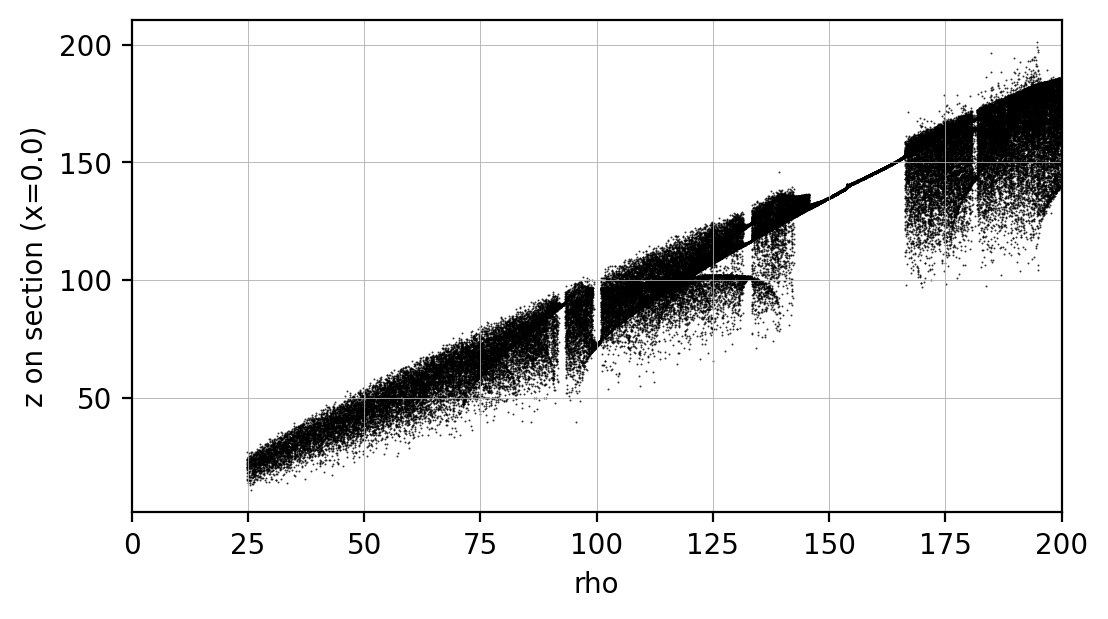
\includegraphics[width=\textwidth]{lorenz_bif_rho.png}
    \caption{Διάγραμμα διακλάδωσης του Lorenz ως προς $\rho$.}
    \label{fig:lorenz-bif-rho}
  \end{subfigure}
  \hfill
  \begin{subfigure}{0.49\textwidth}
    \centering
    \includegraphics[width=\textwidth]{lya_lorenz_rho.png}
    \caption{Διάγραμμα μέγιστου εκθέτη Lyapunov ως προς $\rho$.}
    \label{fig:lorenz-lyap-rho}
  \end{subfigure}
  \caption{Σύγκριση διαγράμματος διακλάδωσης και διαγράμματος Lyapunov για το σύστημα Lorenz ως προς την παράμετρο $\rho$.}
  \label{fig:lorenz-bif-vs-lyap}
\end{figure}

\chapter{Υπολογιστική και Προγραμματιστική Υλοποίηση του Προσομοιωτή}
\label{ch:computational-implementation}

\noindent\textbf{Σύνοψη Κεφαλαίου}.
Το κεφάλαιο αυτό δείχνει πώς περνάμε από τη διεπαφή του προσομοιωτή στον
αριθμητικό πυρήνα. Πρώτα παρουσιάζονται η τεχνολογική στοίβα και η βασική
αρχιτεκτονική της εφαρμογής, έπειτα η ροή χρήσης των tabs και τέλος οι κύριες
εκτελεστικές διαδρομές για τροχιές, διαγράμματα διακλάδωσης και φάσματα
Lyapunov. Οι πιο τεχνικές λεπτομέρειες για πολυπλοκότητα, μνήμη και
Numba/JIT δίνονται στο Παράρτημα.

\section{Σκοπός του κεφαλαίου}
\label{sec:ch2-purpose}

Το πρώτο κεφάλαιο ασχολήθηκε κυρίως με τις έννοιες και τα βασικά εργαλεία της
ανάλυσης. Στο παρόν κεφάλαιο το ενδιαφέρον μεταφέρεται στον τρόπο με τον οποίο
αυτές οι έννοιες υλοποιούνται σε λογισμικό.

Ο στόχος εδώ δεν είναι να παρουσιαστεί όλος ο κώδικας γραμμή προς γραμμή.
Στόχος είναι να γίνει σαφές:
\begin{itemize}
\item ποια είναι τα βασικά μέρη της εφαρμογής,
\item πώς ο χρήστης δίνει τις ρυθμίσεις ενός πειράματος,
\item πώς οι ρυθμίσεις αυτές φτάνουν στον αριθμητικό πυρήνα,
\item και ποια στοιχεία της τρέχουσας υλοποίησης βοηθούν την επεκτασιμότητα και
την αναπαραγωγιμότητα του εργαλείου.
\end{itemize}

Η περιγραφή βασίζεται στο πραγματικό codebase του έργου και όχι σε θεωρητικό
σχήμα ανεξάρτητο από την υλοποίηση
\cite{nlds_internal_md_docs,nlds_src_app_main}.

\section{Υπολογιστική στοίβα και αρχιτεκτονική}
\label{sec:ch2-stack-architecture}

Ο προσομοιωτής υλοποιείται σε Python και συνδυάζει εργαλεία για διεπαφή
χρήστη, αριθμητική ολοκλήρωση, συμβολικό χειρισμό εξισώσεων και παραγωγή
διαγραμμάτων. Η βασική στοίβα συνοψίζεται στον Πίνακα~\ref{tab:ch2-stack}.

\begin{table}[H]
\centering
\caption{Κύρια τεχνολογική στοίβα του προσομοιωτή}
\label{tab:ch2-stack}
\renewcommand{\arraystretch}{1.15}
\begin{tabular}{|l|p{0.64\textwidth}|}
\hline
\textbf{Συστατικό} & \textbf{Ρόλος στην υλοποίηση} \\
\hline
Python & Κεντρική γλώσσα υλοποίησης για διεπαφή, έλεγχο ροής, αριθμητική και exports. \\
\hline
Streamlit & Γραφικό περιβάλλον με tabs, widgets και \texttt{session\_state}. \\
\hline
NumPy & Πίνακες κατάστασης, διανυσματική αριθμητική και αριθμητική επεξεργασία δεδομένων. \\
\hline
SciPy (\texttt{solve\_ivp}) & Προσαρμοστικοί ολοκληρωτές RK45 και DOP853, καθώς και event detection. \\
\hline
SymPy & Parsing custom εξισώσεων, symbolic Jacobian και expression-based τομές Poincar\'e. \\
\hline
Numba & Επιτάχυνση fixed-step kernels, Lyapunov loops και sweep backends. \\
\hline
Pandas & Δομές δεδομένων για sweeps και εξαγωγές πινάκων. \\
\hline
Matplotlib & Διαγράμματα φάσης, χρονοσειρές, bifurcation και Lyapunov. \\
\hline
\end{tabular}
\end{table}

Η στοίβα αυτή φαίνεται άμεσα στα αρχεία εξαρτήσεων και στα κύρια modules της
εφαρμογής \cite{nlds_src_app_requirements,nlds_src_app_main}.

\begin{importantbox}
\textbf{Βασικός αρχιτεκτονικός διαχωρισμός}

\begin{itemize}
\item \textbf{Διεπαφή χρήστη:} \path{app/nlds_app.py} και
\path{app/ui/bifurcation_tab.py}. Εδώ ο χρήστης ορίζει το σύστημα, τους
χρόνους ολοκλήρωσης και τις ρυθμίσεις των διαγραμμάτων.
\item \textbf{Ορχήστρωση και cache:} \path{app/cache.py},
\path{app/logic/}, \path{app/sweep.py}, \path{app/export_utils.py}.
Εδώ γίνεται ο έλεγχος των ρυθμίσεων, η αποθήκευση ενδιάμεσων αποτελεσμάτων και
η επιλογή της κατάλληλης διαδρομής εκτέλεσης.
\item \textbf{Αριθμητικός πυρήνας:} \path{core/solver.py},
\path{core/symplectic_solver.py}, \path{core/poincare_sweep.py},
\path{core/lyapunov.py}, \path{core/numba_backend/}. Εδώ βρίσκονται οι
ολοκληρωτές και οι βασικοί αλγόριθμοι.
\end{itemize}
\end{importantbox}

Ο παραπάνω διαχωρισμός επιτρέπει να αλλάξει ο τρόπος εκτέλεσης ενός αριθμητικού
βρόχου χωρίς να χρειαστεί να αλλάξει η διεπαφή του χρήστη
\cite{nlds_src_app_main,nlds_src_ui_bifurcation_tab,nlds_src_app_cache,nlds_src_core_solver,nlds_src_core_lyapunov}.

\begin{figure}[H]
\centering
\fbox{\parbox[c][4.0cm][c]{0.88\textwidth}{\centering
Placeholder\\
Σχηματική ροή αρχιτεκτονικής:\\
sidebar / tabs $\rightarrow$ objects ρυθμίσεων $\rightarrow$ cache/orchestration
$\rightarrow$ numerical core}}
\caption{Placeholder για συνολικό διάγραμμα ροής της αρχιτεκτονικής του προσομοιωτή.}
\label{fig:ch2-architecture-placeholder}
\end{figure}

\section{Ροή χρήσης της εφαρμογής}
\label{sec:ch2-ui-flow}

\subsection{Ορισμός συστήματος και αρχικών δεδομένων}
\label{subsec:ch2-system-setup}

Η πρώτη επαφή του χρήστη με την εφαρμογή γίνεται από το sidebar. Εκεί
επιλέγεται αν θα χρησιμοποιηθεί ένα από τα έτοιμα συστήματα ή ένα custom
σύστημα, ποιες είναι οι αρχικές συνθήκες και ποιος solver θα χρησιμοποιηθεί.

\begin{guidebox}
Στην αρχική ρύθμιση του προβλήματος ο χρήστης δίνει:
\begin{enumerate}
\item το είδος του συστήματος,
\item τις παραμέτρους του μοντέλου,
\item τις αρχικές συνθήκες,
\item και, στην custom περίπτωση, τα ονόματα μεταβλητών και τις εξισώσεις.
\end{enumerate}
\end{guidebox}

Για custom συστήματα η εφαρμογή επιτρέπει και symbolic παραγωγή Ιακωβιανού,
ώστε ο ίδιος ο χρήστης να επιλέξει αργότερα αν θα χρησιμοποιηθεί αναλυτικός ή
αριθμητικός Jacobian στους υπολογισμούς Lyapunov
\cite{nlds_src_app_main,nlds_src_app_numba_custom,nlds_src_core_lyapunov}.

\begin{figure}[H]
\centering
\begin{subfigure}{0.32\textwidth}
  \centering
  \includegraphics[width=\textwidth]{figures/ch2/s1_system_selection.png}
  \caption{Επιλογή συστήματος και solver kind.}
  \label{fig:ch2-s1-system}
\end{subfigure}
\hfill
\begin{subfigure}{0.32\textwidth}
  \centering
  \includegraphics[width=\textwidth]{figures/ch2/s2_initial_and_custom_definitions.png}
  \caption{Αρχικές συνθήκες και custom εξισώσεις.}
  \label{fig:ch2-s2-custom-def}
\end{subfigure}
\hfill
\begin{subfigure}{0.32\textwidth}
  \centering
  \includegraphics[width=\textwidth]{figures/ch2/s3_symbolic_jacobian.png}
  \caption{Προβολή symbolic Jacobian.}
  \label{fig:ch2-s3-jacobian}
\end{subfigure}
\caption{Βασικά βήματα ορισμού του συστήματος στο sidebar και στα πρώτα blocks της εφαρμογής.}
\label{fig:ch2-tab-setup}
\end{figure}

\subsection{Ολοκλήρωση τροχιάς και οπτικοποίηση}
\label{subsec:ch2-integration-visualization}

Αφού οριστεί το πρόβλημα, ο χρήστης επιλέγει το χρονικό παράθυρο ολοκλήρωσης,
το βήμα \(\Delta t\), τους άξονες προβολής και τις ανοχές του solver όπου αυτό
χρειάζεται. Η βασική χρονική δειγματοληψία γράφεται ως
\begin{equation}
t_k=t_0+k\Delta t,
\qquad k=0,1,\dots,N.
\end{equation}
Με αυτά τα δεδομένα παράγονται η τροχιά αναφοράς, το φασικό πορτρέτο και οι
χρονοσειρές.

\begin{guidebox}
Στο πρώτο tab συγκεντρώνονται οι ρυθμίσεις που αφορούν:
\begin{enumerate}
\item τον χρόνο ολοκλήρωσης,
\item τις παραμέτρους του συστήματος,
\item την αφαίρεση του μεταβατικού μέρους,
\item την προβολή σε 2D ή 3D άξονες,
\item και την αποθήκευση των ρυθμίσεων του run.
\end{enumerate}
\end{guidebox}

\begin{figure}[H]
\centering
\begin{subfigure}{0.32\textwidth}
  \centering
  \includegraphics[width=\textwidth]{figures/ch2/s4_integration_controls.png}
  \caption{Χρονικό παράθυρο ολοκλήρωσης.}
  \label{fig:ch2-s4-integration}
\end{subfigure}
\hfill
\begin{subfigure}{0.32\textwidth}
  \centering
  \includegraphics[width=\textwidth]{figures/ch2/s5_system_parameters_custom.png}
  \caption{Παράμετροι συστήματος.}
  \label{fig:ch2-s5-params}
\end{subfigure}
\hfill
\begin{subfigure}{0.32\textwidth}
  \centering
  \includegraphics[width=\textwidth]{figures/ch2/s6_plot_settings_lyapunov.png}
  \caption{Plot και Lyapunov settings.}
  \label{fig:ch2-s6-plot}
\end{subfigure}
\caption{Κύριες ρυθμίσεις ολοκλήρωσης και post-processing στο πρώτο tab.}
\label{fig:ch2-tab1-top}
\end{figure}

\begin{figure}[H]
\centering
\begin{subfigure}{0.32\textwidth}
  \centering
  \includegraphics[width=\textwidth]{figures/ch2/s7_axis_selection.png}
  \caption{Επιλογή αξόνων.}
  \label{fig:ch2-s7-axis}
\end{subfigure}
\hfill
\begin{subfigure}{0.32\textwidth}
  \centering
  \includegraphics[width=\textwidth]{figures/ch2/s8_solver_tolerances.png}
  \caption{Ανοχές solver.}
  \label{fig:ch2-s8-tols}
\end{subfigure}
\hfill
\begin{subfigure}{0.32\textwidth}
  \centering
  \includegraphics[width=\textwidth]{figures/ch2/s9_save_configuration.png}
  \caption{Αποθήκευση configuration.}
  \label{fig:ch2-s9-save}
\end{subfigure}
\caption{Ρυθμίσεις προβολής, ανοχών και αποθήκευσης του run.}
\label{fig:ch2-tab1-bottom}
\end{figure}

Το δεύτερο tab δεν λύνει ξανά το πρόβλημα από την αρχή. Πατά πάνω στην ήδη
υπολογισμένη τροχιά και επιτρέπει να επιλεγεί ένα μικρότερο χρονικό παράθυρο
για καθαρότερη απεικόνιση των χρονοσειρών
\cite{nlds_src_app_main}.

\begin{figure}[H]
\centering
\includegraphics[width=0.56\textwidth]{figures/ch2/s10_time_series_window.png}
\caption{Το δεύτερο tab επιτρέπει επιλογή χρονικού παραθύρου πάνω στην ήδη
υπολογισμένη χρονοσειρά.}
\label{fig:ch2-s10-ts}
\end{figure}

\subsection{Παραμετρικές σαρώσεις}
\label{subsec:ch2-sweeps-ui}

Στο τρίτο tab ο χρήστης δεν ακολουθεί μία μόνο τροχιά, αλλά επαναλαμβάνει την
ολοκλήρωση για πολλές τιμές μιας παραμέτρου. Αν η παράμετρος γραφεί ως
\(\mu\), τότε τα σημεία της σάρωσης δίνονται από τη σχέση
\begin{equation}
\mu_i=\mu_{\min}+i\,\Delta\mu.
\end{equation}
Για κάθε τιμή της παραμέτρου παράγεται είτε σύνολο σημείων για διάγραμμα
διακλάδωσης είτε ένα φάσμα εκθετών Lyapunov.

\begin{guidebox}
Το τρίτο tab χωρίζεται λειτουργικά σε δύο μέρη:
\begin{enumerate}
\item ρυθμίσεις για bifurcation sweep με τομή Poincar\'e ή local extrema,
\item ρυθμίσεις για Lyapunov sweep με QR interval και κανόνες clipping.
\end{enumerate}
\end{guidebox}

\begin{figure}[H]
\centering
\begin{subfigure}{0.32\textwidth}
  \centering
  \includegraphics[width=\textwidth]{figures/ch2/s11_tab3_top_setup.png}
  \caption{Γενικές ρυθμίσεις sweep.}
  \label{fig:ch2-s11-tab3-top}
\end{subfigure}
\hfill
\begin{subfigure}{0.32\textwidth}
  \centering
  \includegraphics[width=\textwidth]{figures/ch2/s12_bifurcation_parallel_section.png}
  \caption{Ρυθμίσεις bifurcation sweep.}
  \label{fig:ch2-s12-bif-section}
\end{subfigure}
\hfill
\begin{subfigure}{0.32\textwidth}
  \centering
  \includegraphics[width=\textwidth]{figures/ch2/s13_bifurcation_method_earlystop.png}
  \caption{Method και early stop.}
  \label{fig:ch2-s13-bif-method}
\end{subfigure}
\caption{Κύριες επιλογές για bifurcation sweep στο τρίτο tab.}
\label{fig:ch2-tab3-top}
\end{figure}

\begin{figure}[H]
\centering
\begin{subfigure}{0.48\textwidth}
  \centering
  \includegraphics[width=\textwidth]{figures/ch2/s14_lyapunov_sweep_settings.png}
  \caption{Ρυθμίσεις Lyapunov sweep.}
  \label{fig:ch2-s14-lya-settings}
\end{subfigure}
\hfill
\begin{subfigure}{0.48\textwidth}
  \centering
  \includegraphics[width=\textwidth]{figures/ch2/s15_lyapunov_clip_and_run.png}
  \caption{Clipping και εκτέλεση sweep.}
  \label{fig:ch2-s15-lya-run}
\end{subfigure}
\caption{Ρυθμίσεις Lyapunov sweep στο τρίτο tab.}
\label{fig:ch2-tab3-bottom}
\end{figure}

\section{Από τη διεπαφή στον αριθμητικό πυρήνα}
\label{sec:ch2-ui-to-core}

\begin{definitionbox}{Objects ρυθμίσεων του run}{nlds_src_app_params}
Οι βασικές ρυθμίσεις ενός run συγκεντρώνονται σε μικρά dataclasses. Τα πιο
κεντρικά είναι τα \texttt{SystemConfig}, \texttt{InitialConditions},
\texttt{IntegrationConfig}, \texttt{SolverTolerances},
\texttt{SweepRunConfig} και \texttt{LyapunovConfig}. Με αυτόν τον τρόπο η
εφαρμογή μεταφέρει οργανωμένα τα δεδομένα από τη διεπαφή στον πυρήνα.
\end{definitionbox}

Στην πράξη, ο χρήστης δεν επικοινωνεί απευθείας με τις numerical routines.
Πρώτα δημιουργούνται τα objects των ρυθμίσεων και έπειτα επιλέγεται το σωστό
μονοπάτι εκτέλεσης.

\begin{importantbox}
\textbf{Οι τρεις βασικές εκτελεστικές διαδρομές}

\begin{itemize}
\item \textbf{Μοναδική τροχιά:}
\path{app/nlds_app.py}
\(\rightarrow\)
\path{app/cache.py:solve_cached}
\(\rightarrow\)
\path{core/solver.py} ή \path{core/symplectic_solver.py}.
\item \textbf{Μεμονωμένος υπολογισμός Lyapunov:}
\path{app/nlds_app.py}
\(\rightarrow\)
\path{app/logic/lyapunov_cached.py}
\(\rightarrow\)
\path{core/lyapunov.py}.
\item \textbf{Sweep παραμέτρων:}
\path{app/ui/bifurcation_tab.py}
\(\rightarrow\)
\path{app/sweep.py} ή \path{app/logic/lyapunov_sweep.py}
\(\rightarrow\)
\path{core/poincare_sweep.py} ή \path{core/lyapunov.py}.
\end{itemize}
\end{importantbox}

\subsection{Μοναδική τροχιά}
\label{subsec:ch2-single-run-path}

Για ένα απλό run, η διεπαφή συγκεντρώνει τα στοιχεία του προβλήματος και
καλεί τη συνάρτηση \texttt{solve\_cached}. Η συνάρτηση αυτή αποφασίζει αν θα
χρησιμοποιηθεί adaptive solver, fixed-step RK4 ή symplectic ολοκληρωτής,
ανάλογα με το \texttt{solver\_kind} και το είδος του συστήματος
\cite{nlds_src_app_cache,nlds_src_core_solver,nlds_src_core_symplectic}.

Στο σημείο αυτό εμφανίζεται και το πρώτο απλό μαθηματικό φίλτρο της
υλοποίησης: σε χαμιλτονιανά runs το state πρέπει να μπορεί να γραφεί ως
\([\mathbf{q},\mathbf{p}]\), δηλαδή ως ζεύγος γενικευμένων θέσεων και ορμών.
Γι' αυτό ο symplectic solver ενεργοποιείται μόνο όταν ο αριθμός μεταβλητών
είναι άρτιος και το σύστημα έχει την κατάλληλη μορφή.

\subsection{Υπολογισμός φάσματος Lyapunov}
\label{subsec:ch2-lyapunov-path}

Για τους εκθέτες Lyapunov η διεπαφή χρησιμοποιεί διαφορετικό μονοπάτι. Το
\path{app/logic/lyapunov_cached.py} προετοιμάζει το σύστημα, επιλέγει αν θα
χρησιμοποιηθεί analytic ή finite-difference Jacobian και τελικά καλεί το
\path{core/lyapunov.py} \cite{nlds_src_logic_lyapunov_cached,nlds_src_core_lyapunov}.

Η πιο βασική χρονική ρύθμιση εδώ είναι το QR interval. Αν \(\Delta t\) είναι
το αριθμητικό βήμα και \(q\) το πλήθος βημάτων ανά ορθοκανονικοποίηση, τότε
\begin{equation}
\Delta T_{\mathrm{QR}} = q\,\Delta t.
\end{equation}
Η σχέση αυτή χρησιμοποιείται άμεσα από τον κώδικα για να περάσουμε από τη
ρύθμιση της διεπαφής στο πραγματικό αριθμητικό χρονοδιάστημα του υπολογισμού.

\subsection{Sweeps παραμέτρων}
\label{subsec:ch2-sweep-path}

Στα sweeps το ίδιο πείραμα επαναλαμβάνεται πολλές φορές. Στο bifurcation μέρος
του τρίτου tab, η \texttt{run\_sweep\_chunk} συλλέγει είτε τομές Poincar\'e
είτε local extrema, ανάλογα με τη ρύθμιση που επέλεξε ο χρήστης
\cite{nlds_src_ui_bifurcation_tab,nlds_src_app_sweep,nlds_src_core_poincare}.

Στο Lyapunov sweep, η ροή είναι αντίστοιχη αλλά ο τελικός στόχος δεν είναι ένα
σύνολο σημείων τομής. Για κάθε τιμή της παραμέτρου υπολογίζεται ένα φάσμα
εκθετών και αποθηκεύεται συνήθως ο μεγαλύτερος εκθέτης ή το πλήρες διάνυσμα,
ανάλογα με το mode της εκτέλεσης
\cite{nlds_src_logic_lyapunov_sweep,nlds_src_core_lyapunov}.

\section{Νεότερα στοιχεία της τρέχουσας υλοποίησης}
\label{sec:ch2-current-implementation}

Το σημερινό codebase έχει αρκετά στοιχεία που δεν φαίνονται αμέσως από το
θεωρητικό κεφάλαιο, αλλά είναι σημαντικά για την πρακτική λειτουργία της
εφαρμογής.

\subsection{Φραγμένη αποθήκευση τροχιάς}
\label{subsec:ch2-bounded-trajectory}

Σε ένα μεγάλο run δεν είναι πάντα χρήσιμο να αποθηκεύονται όλα τα σημεία της
τροχιάς. Για τον λόγο αυτό το \texttt{IntegrationConfig} περιλαμβάνει την
παράμετρο \texttt{max\_store\_steps}. Έτσι, ο solver μπορεί να ολοκληρώνει σε
μεγάλο χρονικό διάστημα, αλλά η μνήμη που δεσμεύεται για το τελικό αποθηκευμένο
αποτέλεσμα να παραμένει ελεγχόμενη
\cite{nlds_src_app_params,nlds_src_app_cache,nlds_src_core_solver,nlds_src_core_symplectic}.

Η ίδια λογική συνεχίζεται και στην οπτικοποίηση, όπου το plotting
χρησιμοποιεί decimation ώστε να μη στέλνονται στο γράφημα πολύ περισσότερα
σημεία από όσα μπορούν να διαβαστούν εύκολα.

\subsection{Μεγάλα sweeps με bounded memory}
\label{subsec:ch2-bounded-sweeps}

Στα μεγάλα bifurcation sweeps, η εφαρμογή δεν κρατά απεριόριστα όλες τις
παλιές γραμμές στη RAM. Διατηρεί ένα πρόσφατο κομμάτι δεδομένων σε πλήρη
ανάλυση και ένα reservoir sample από παλαιότερα σημεία, ώστε το διάγραμμα να
μένει αντιπροσωπευτικό χωρίς να μεγαλώνει απεριόριστα η μνήμη
\cite{nlds_src_ui_bifurcation_tab,nlds_src_logic_reservoir}.

Η λεπτομερής ανάλυση μνήμης για αυτά τα σημεία δίνεται στο
Παράρτημα~\ref{app:ch2-memory}.

\subsection{Αποθήκευση ρυθμίσεων και αναπαραγωγιμότητα}
\label{subsec:ch2-reproducibility}

Η εφαρμογή επιτρέπει αποθήκευση τόσο ενός απλού run όσο και ενός sweep σε
μορφή JSON. Το \texttt{app/export\_utils.py} κατασκευάζει οργανωμένα blocks με
πληροφορίες για το σύστημα, τις αρχικές συνθήκες, τον solver, τα post-process
settings και, όταν είναι διαθέσιμο, το commit του repository
\cite{nlds_src_app_export}.

Αυτό είναι χρήσιμο γιατί το αποτέλεσμα ενός πειράματος δεν εξαρτάται μόνο από
τις εξισώσεις. Εξαρτάται επίσης από:
\begin{itemize}
\item το \(\Delta t\),
\item το transient cut,
\item τις ανοχές του solver,
\item το QR interval,
\item και το mode του sweep.
\end{itemize}

Με την αποθήκευση αυτών των ρυθμίσεων το πείραμα μπορεί να επαναληφθεί πολύ πιο
αξιόπιστα.

\subsection{Compiled paths και ασφαλή fallbacks}
\label{subsec:ch2-numba-short}

Η εφαρμογή δεν τρέχει όλον τον κώδικα σε compiled μορφή. Η διεπαφή, ο έλεγχος
ροής και η παραγωγή γραφημάτων παραμένουν σε Python. Εκεί που χρειάζεται
επιτάχυνση, ενεργοποιούνται Numba kernels για fixed-step RK4, symplectic runs,
Lyapunov υπολογισμούς και ορισμένα sweep backends
\cite{nlds_src_core_numba,nlds_src_app_numba_custom}.

Αν το compiled μονοπάτι δεν είναι διαθέσιμο ή αν μια custom περίπτωση δεν
μπορεί να μεταγλωττιστεί με ασφάλεια, ο κώδικας επιστρέφει στην κανονική
Python διαδρομή. Με αυτόν τον τρόπο η εφαρμογή παραμένει λειτουργική χωρίς να
θυσιάζει τη γενικότητα των custom ορισμών.

Η πιο τεχνική περιγραφή των compiled paths δίνεται στο
Παράρτημα~\ref{app:ch2-numba}.

\section{Συνολική εικόνα του κεφαλαίου}
\label{sec:ch2-closing}

Το βασικό συμπέρασμα του κεφαλαίου είναι ότι ο προσομοιωτής δεν είναι απλώς ένα
σύνολο μεμονωμένων scripts. Είναι μια ενιαία ροή εργασίας στην οποία:
\begin{itemize}
\item η διεπαφή συγκεντρώνει οργανωμένα τις ρυθμίσεις,
\item το layer ορχήστρωσης επιλέγει το κατάλληλο μονοπάτι εκτέλεσης,
\item και ο αριθμητικός πυρήνας εκτελεί το ουσιαστικό υπολογιστικό έργο.
\end{itemize}

Η κύρια ροή κρατήθηκε εδώ όσο γίνεται απλή. Οι αναλυτικότεροι τύποι
πολυπλοκότητας, τα όρια μνήμης και η τεχνική περιγραφή της Numba/JIT
υλοποίησης μεταφέρονται στο επόμενο παράρτημα.


\appendix

\chapter*{Παραρτήματα}
\addcontentsline{toc}{chapter}{Παραρτήματα}
\setcounter{section}{0}
\newcommand{\appendixletter}[1]{%
  \ifcase#1%
  \or A\or B\or C\or D\or E\or F\or G\or H\or I\or J%
  \else #1%
  \fi%
}
\renewcommand{\thesection}{\appendixletter{\value{section}}}
\renewcommand{\thesubsection}{\thesection.\arabic{subsection}}

\section{Σύνοψη διεπαφής και συμβάσεων δεδομένων του \texttt{solver.py}}
\label{app:solver-interface}
\begin{importantbox}
Ο \texttt{solver.py} ορίζει ένα ελαφρύ δοχείο αποτελέσματος
(\texttt{OdeSolution}) και δύο βασικούς ολοκληρωτές:
\begin{itemize}
\item \texttt{integrate\_system}: επίλυση IVP μέσω
\texttt{scipy.integrate.solve\_ivp} και επιστροφή δειγματοληπτημένων τιμών.
\item \texttt{integrate\_system\_rk4}: σταθερού βήματος κλασικό RK4 για
ελεγχόμενη και αναπαραγώγιμη σύγκριση.
\end{itemize}
Η έξοδος έχει τη μορφή
\begin{equation*}
t \in \mathbb{R}^{N}, \qquad y \in \mathbb{R}^{d \times N},
\end{equation*}
ώστε ένα διάγραμμα φάσης $y_i$-$y_j$ να υλοποιείται άμεσα από τα ζεύγη
$(y_i(t_k),y_j(t_k))$.
\end{importantbox}

\section{Τύποι των αριθμητικών μεθόδων}

\subsection{Runge-Kutta 4ης τάξης σταθερού βήματος}
\label{app:rk4-formula}
Η μέθοδος RK4 γράφεται
\begin{equation}
\mathbf{x}_{k+1}=\mathbf{x}_k+\frac{\Delta t}{6}\left(\mathbf{k}_1+2\mathbf{k}_2+2\mathbf{k}_3+\mathbf{k}_4\right),
\end{equation}
όπου
\begin{equation}
\mathbf{k}_1=f(t_k,\mathbf{x}_k),\quad
\mathbf{k}_2=f\!\left(t_k+\frac{\Delta t}{2},\mathbf{x}_k+\frac{\Delta t}{2}\mathbf{k}_1\right),
\end{equation}
\begin{equation}
\mathbf{k}_3=f\!\left(t_k+\frac{\Delta t}{2},\mathbf{x}_k+\frac{\Delta t}{2}\mathbf{k}_2\right),\quad
\mathbf{k}_4=f\!\left(t_k+\Delta t,\mathbf{x}_k+\Delta t\,\mathbf{k}_3\right).
\end{equation}

\subsection{Προσαρμοστικό Runge-Kutta: RK45 και DOP853}
\label{app:adaptive-rk-formulas}
Για ένα γενικό embedded Runge-Kutta βήμα υπολογίζονται στάδια
\begin{equation}
\mathbf{k}_i=\mathbf{f}\!\left(t_k+c_i h_k,\;\mathbf{x}_k+h_k\sum_{j=1}^{i-1}a_{ij}\mathbf{k}_j\right),
\qquad i=1,\dots,s.
\end{equation}

Στην RK45 κατασκευάζονται δύο προσεγγίσεις στο ίδιο βήμα,
\begin{equation}
\mathbf{x}_{k+1}^{(5)}=\mathbf{x}_k+h_k\sum_{i=1}^{s}b_i^{(5)}\mathbf{k}_i,
\qquad
\mathbf{x}_{k+1}^{(4)}=\mathbf{x}_k+h_k\sum_{i=1}^{s}b_i^{(4)}\mathbf{k}_i,
\end{equation}
και η διαφορά τους
\begin{equation}
\boldsymbol{\varepsilon}_k=\mathbf{x}_{k+1}^{(5)}-\mathbf{x}_{k+1}^{(4)}
\end{equation}
χρησιμοποιείται ως εκτιμητής τοπικού σφάλματος. Το επόμενο βήμα προσαρμόζεται
τυπικά ως
\begin{equation}
h_{k+1}=\eta\,h_k\left(\frac{\mathrm{tol}}{\|\boldsymbol{\varepsilon}_k\|}\right)^{\!1/5}.
\end{equation}

Αντίστοιχα, στον DOP853:
\begin{equation}
\mathbf{x}_{k+1}^{(8)}=\mathbf{x}_k+h_k\sum_{i=1}^{s}b_i^{(8)}\mathbf{k}_i,
\qquad
\mathbf{x}_{k+1}^{(\mathrm{emb})}=\mathbf{x}_k+h_k\sum_{i=1}^{s}\widehat b_i\mathbf{k}_i,
\end{equation}
\begin{equation}
\boldsymbol{\varepsilon}_k^{\mathrm{(DOP853)}}=
\mathbf{x}_{k+1}^{(8)}-\mathbf{x}_{k+1}^{(\mathrm{emb})},
\qquad
h_{k+1}=\eta\,h_k\left(\frac{\mathrm{tol}}{\|\boldsymbol{\varepsilon}_k^{\mathrm{(DOP853)}}\|}\right)^{\!1/9}.
\end{equation}

\subsection{Verlet και Forest-Ruth για Χαμιλτονιανά συστήματα}
\label{app:symplectic-formulas}
Για Χαμιλτονιανό σύστημα με
\begin{equation}
\dot{\mathbf{q}}=\frac{\partial H}{\partial \mathbf{p}},\qquad
\dot{\mathbf{p}}=-\frac{\partial H}{\partial \mathbf{q}},
\end{equation}
ένα βήμα St\"ormer-Verlet μήκους $h$ γράφεται
\begin{equation}
\mathbf{p}_{n+1/2}=\mathbf{p}_n-\frac{h}{2}\nabla V(\mathbf{q}_n),
\qquad
\mathbf{q}_{n+1}=\mathbf{q}_n+h\nabla_{\mathbf{p}}T(\mathbf{p}_{n+1/2}),
\end{equation}
\begin{equation}
\mathbf{p}_{n+1}=\mathbf{p}_{n+1/2}-\frac{h}{2}\nabla V(\mathbf{q}_{n+1}).
\end{equation}

Αν συμβολίσουμε με $\Phi_h^{\mathrm{SV}}$ τον χάρτη που παίρνει την κατάσταση
$\mathbf{z}_n=(\mathbf{q}_n,\mathbf{p}_n)$ και την μεταφέρει στην επόμενη
κατάσταση $\mathbf{z}_{n+1}$ μετά από ένα βήμα St\"ormer-Verlet μήκους $h$,
τότε ο Forest-Ruth 4ης τάξης γράφεται ως σύνθεση τέτοιων χαρτών. Το σύμβολο
$\circ$ σημαίνει διαδοχική εφαρμογή: πρώτα εφαρμόζεται ο δεξιότερος χάρτης και
μετά ο επόμενος προς τα αριστερά.

Με αυτή τη σημειογραφία, ο Forest-Ruth 4ης τάξης κατασκευάζεται ως σύνθεση
τριών βημάτων Verlet:
\begin{equation}
\Phi_h^{\mathrm{FR}}=
\Phi_{w_1 h}^{\mathrm{SV}}\circ
\Phi_{w_0 h}^{\mathrm{SV}}\circ
\Phi_{w_1 h}^{\mathrm{SV}},
\end{equation}
με
\begin{equation}
w_1=\frac{1}{2-2^{1/3}},
\qquad
w_0=-\frac{2^{1/3}}{2-2^{1/3}}.
\end{equation}

\section{Ψευδοκώδικας βασικών ολοκληρωτών}

\subsection*{Fixed-step RK4}
\begin{algorithm}[H]
\caption{\texttt{integrate\_system\_rk4}}
\label{alg:rk4-fixed-tuned}
\begingroup
\small
\setlength{\parskip}{0pt}
\begin{algorithmic}[1]
\Require RHS $f(t,\mathbf{y})$, $[t_0,t_f]$, $\mathbf{y}_0$, step $h$
\Ensure Time grid and state history
\State Convert $\mathbf{y}_0$ to float array
\State Compute number of steps and allocate arrays
\For{$i=1,\dots,N-1$}
  \State Compute $\mathbf{k}_1,\mathbf{k}_2,\mathbf{k}_3,\mathbf{k}_4$
  \State Update state using
  \Statex \hspace{\algorithmicindent} $Y[:,i] \gets \mathbf{y}_i + \tfrac{h}{6}\left(\mathbf{k}_1 + 2\mathbf{k}_2\right.$
  \Statex \hspace{2\algorithmicindent} $\left.+\,2\mathbf{k}_3 + \mathbf{k}_4\right)$
  \State Update time $t[i] \gets t[i-1] + h$
\EndFor
\State Return solution arrays
\end{algorithmic}
\endgroup
\end{algorithm}

\subsection*{Ολοκλήρωση τροχιάς για φασικά διαγράμματα}
\begin{algorithm}[H]
\caption{Trajectory integration for phase portraits}
\label{alg:traj-phase-tuned}
\begin{tcolorbox}[appendixalgobox]
\begin{algorithmic}[1]
\Require $f(t,\mathbf{x})$, $[t_0,t_f]$, $\mathbf{x}_0$, $\Delta t$
\Ensure Arrays $\{t_k\}$ and $\{\mathbf{x}(t_k)\}$
\State Construct evaluation grid $t_k = t_0 + k\Delta t$
\State Solve IVP to obtain $\mathbf{x}(t_k)$
\State Return arrays $\{t_k\}$ and $\{\mathbf{x}(t_k)\}$
\end{algorithmic}
\end{tcolorbox}
\end{algorithm}

\subsection*{Symplectic Forest-Ruth 4ης τάξης}
\begin{algorithm}[H]
\caption{\texttt{integrate\_system\_symplectic\_fr}}
\label{alg:fr4-tuned}
\begin{tcolorbox}[appendixalgobox]
\begin{algorithmic}[1]
\Require Separable Hamiltonian state $\mathbf{z}=[\mathbf{q},\mathbf{p}]$, $[t_0,t_f]$, step $h$
\Ensure Symplectic time evolution
\State Define coefficients $c_1,c_2,c_3$ of Forest-Ruth
\State Define auxiliary \texttt{VerletStep}
\For{$i=1,\dots,N-1$}
  \State Split current state into $(\mathbf{q},\mathbf{p})$
  \State Apply \texttt{VerletStep} with $c_1h$
  \State Apply \texttt{VerletStep} with $c_2h$
  \State Apply \texttt{VerletStep} with $c_3h$
  \State Store new state
\EndFor
\State Return solution arrays
\end{algorithmic}
\end{tcolorbox}
\end{algorithm}

\section{Επιλογές δειγματοληψίας και αναπαραγωγιμότητα}
\label{app:sampling}
Ο αριθμός σημείων δειγματοληψίας καθορίζεται από το \texttt{t\_step} ή
ισοδύναμα από το πλήθος βημάτων και κατασκευάζεται ως ισαπέχον πλέγμα στο
$[t_0,t_f]$. Αυτό εξασφαλίζει σταθερή χρονική βάση για χρονοσειρές και
διαγράμματα φάσης, ώστε διαφορετικές εκτελέσεις να μπορούν να συγκρίνονται με
συνεπή τρόπο.

\section{Έλεγχοι ορθότητας εισόδων και ασφαλείς προεπιλογές}
\label{app:input-checks}
Ο κώδικας περιλαμβάνει βασικούς ελέγχους εγκυρότητας, όπως
\texttt{t\_step > 0}, και ενιαία μετατροπή της αρχικής συνθήκης σε διάνυσμα
\texttt{float}. Επίσης χρησιμοποιούνται σημαίες όπως \texttt{success} και
\texttt{message}, ώστε να αποφεύγεται η παραγωγή παραπλανητικών διαγραμμάτων σε
περίπτωση αποτυχίας ολοκλήρωσης.

\section{Αριθμητική εκτίμηση φάσματος Lyapunov}
\label{app:lyapunov}

Η εκτίμηση των εκθετών Lyapunov βασίζεται στην ταυτόχρονη ολοκλήρωση της
τροχιάς αναφοράς και ενός συστήματος εξισώσεων μεταβολής. Για σύστημα
\begin{equation}
\dot{\mathbf{x}}=\mathbf{f}(\mathbf{x},t),
\end{equation}
μια μικρή διαταραχή $\delta\mathbf{x}(t)$ ικανοποιεί κατά προσέγγιση
\begin{equation}
\dot{\delta\mathbf{x}} = J(\mathbf{x}(t),t)\,\delta\mathbf{x},
\qquad
J(\mathbf{x},t)=\frac{\partial \mathbf{f}}{\partial \mathbf{x}}(\mathbf{x},t).
\end{equation}

Αν συγκεντρώσουμε πολλές ανεξάρτητες διαταραχές σε έναν πίνακα
$Y(t)\in\mathbb{R}^{n\times n}$ με αρχική συνθήκη $Y(t_0)=I$, τότε
\begin{equation}
\dot{Y}=J(\mathbf{x}(t),t)\,Y.
\end{equation}
Έτσι προκύπτει το διευρυμένο σύστημα
\begin{equation}
\begin{cases}
\dot{\mathbf{x}} = \mathbf{f}(\mathbf{x},t),\\
\dot{Y} = J(\mathbf{x}(t),t)\,Y.
\end{cases}
\end{equation}

\subsection{Αναλυτικός και αριθμητικός Jacobian}
\label{app:lyapunov-jacobian}

Όταν είναι διαθέσιμος ο αναλυτικός Ιακωβιανός, χρησιμοποιείται απευθείας στις
εξισώσεις μεταβολής. Διαφορετικά, προσεγγίζεται αριθμητικά με κεντρικές
διαφορές:
\begin{equation}
J_{:,j}(\mathbf{x},t)\approx
\frac{\mathbf{f}(\mathbf{x}+\varepsilon \mathbf{e}_j,t)-\mathbf{f}(\mathbf{x}-\varepsilon \mathbf{e}_j,t)}{2\varepsilon}.
\end{equation}
Η δεύτερη επιλογή είναι πιο γενική, αλλά έχει μεγαλύτερο υπολογιστικό κόστος.

\subsection{QR ορθοκανονικοποίηση και συσσώρευση}
\label{app:lyapunov-qr-details}

Καθώς ο πίνακας $Y(t)$ εξελίσσεται, οι στήλες του τείνουν να ευθυγραμμιστούν
με τη διεύθυνση μέγιστης αύξησης. Για να αποφεύγεται αυτή η εκφύλιση,
εφαρμόζεται περιοδικά αποσύνθεση QR:
\begin{equation}
Y = QR.
\end{equation}
Ο πίνακας $Q$ δίνει νέα ορθοκανονική βάση, ενώ ο πίνακας $R$ κρατά την
πληροφορία για τις τοπικές διαστολές και συστολές. Οι εκθέτες εκτιμώνται από
τη συσσώρευση των διαγωνίων όρων του $R$:
\begin{equation}
\lambda_i \approx \frac{1}{T_{\mathrm{m}}}\sum_k \ln |R_{ii}^{(k)}|,
\qquad i=1,\dots,n.
\end{equation}

\subsection{Μικροπαράδειγμα 2D}
\label{app:lyapunov-2d-example}

Για το γραμμικό σύστημα
\begin{equation}
\dot{\mathbf{x}}=A\mathbf{x},\qquad
A=
\begin{bmatrix}
0.2 & 0\\
0 & -0.1
\end{bmatrix},
\end{equation}
οι πραγματικοί εκθέτες Lyapunov είναι $\lambda_1=0.2$ και $\lambda_2=-0.1$.
Αν εφαρμόσουμε QR υπολογισμό με διάστημα ορθοκανονικοποίησης $\Delta T=1$,
τότε σε κάθε βήμα παίρνουμε
\begin{equation}
R=
\begin{bmatrix}
e^{0.2} & 0\\
0 & e^{-0.1}
\end{bmatrix},
\end{equation}
άρα
\begin{equation}
\log|R_{11}|=0.2,\qquad \log|R_{22}|=-0.1.
\end{equation}
Με επανάληψη πολλών βημάτων, ο μέσος όρος αυτών των ποσοτήτων δίνει ακριβώς
τους δύο εκθέτες.

\subsection{Οπτική εξέλιξη της QR ορθοκανονικοποίησης}
\label{app:lyapunov-qr-figures}

Στα επόμενα σχήματα φαίνεται η QR ορθοκανονικοποίηση σε run του συστήματος
R\"ossler. Τα καρέ δείχνουν πώς ένα νέφος διαταραχών παραμορφώνεται από τη
γραμμικοποιημένη ροή και στη συνέχεια επαναφέρεται σε ορθοκανονική βάση.

\begin{figure}[H]
\centering
\begin{subfigure}[t]{0.499\textwidth}
  \centering
  \includegraphics[width=\textwidth,trim=90 70 90 55,clip]{figures/frame_000_delay-1s.png}
  \caption{chunk=1}
  \label{fig:ch1-cpp-qr-frames-top-1}
\end{subfigure}%
\begin{subfigure}[t]{0.499\textwidth}
  \centering
  \includegraphics[width=\textwidth,trim=90 70 90 55,clip]{figures/frame_001_delay-1s.png}
  \caption{chunk=101}
  \label{fig:ch1-cpp-qr-frames-top-2}
\end{subfigure}
\vspace{0.25em}
\begin{subfigure}[t]{0.78\textwidth}
  \centering
  \includegraphics[width=\textwidth,trim=90 70 90 55,clip]{figures/frame_002_delay-1s.png}
  \caption{chunk=201}
  \label{fig:ch1-cpp-qr-frames-top-3}
\end{subfigure}
\caption{Εξέλιξη της QR ορθοκανονικοποίησης σε αρχικό στάδιο του run \cite{gkountinakos_chaos_trace_cpp_2026}.}
\label{fig:ch1-cpp-qr-frames-top}
\end{figure}

\begin{figure}[H]
\centering
\begin{subfigure}[t]{0.499\textwidth}
  \centering
  \includegraphics[width=\textwidth,trim=90 70 90 55,clip]{figures/frame_003_delay-1s.png}
  \caption{chunk=301}
  \label{fig:ch1-cpp-qr-frames-bottom-1}
\end{subfigure}%
\begin{subfigure}[t]{0.499\textwidth}
  \centering
  \includegraphics[width=\textwidth,trim=90 70 90 55,clip]{figures/frame_004_delay-1s.png}
  \caption{chunk=401}
  \label{fig:ch1-cpp-qr-frames-bottom-2}
\end{subfigure}
\vspace{0.25em}
\begin{subfigure}[t]{0.78\textwidth}
  \centering
  \includegraphics[width=\textwidth,trim=90 70 90 55,clip]{figures/frame_005_delay-1s.png}
  \caption{chunk=501}
  \label{fig:ch1-cpp-qr-frames-bottom-3}
\end{subfigure}
\caption{Εξέλιξη της QR ορθοκανονικοποίησης σε μεταγενέστερο στάδιο του run \cite{gkountinakos_chaos_trace_cpp_2026}.}
\label{fig:ch1-cpp-qr-frames-bottom}
\end{figure}

\subsection{Placeholder για μελέτη επιλογής QR period}
\label{app:lyapunov-qr-period-placeholder}

\begin{center}
\fbox{\parbox[c][4.5cm][c]{0.88\textwidth}{\centering
Placeholder\\
Καμπύλες / heatmaps για τη μελέτη επιλογής QR period\\
(θα προστεθούν όταν οριστικοποιηθούν τα αντίστοιχα exports)}}%
\end{center}

\subsection*{Ψευδοκώδικας: Εκτίμηση φάσματος Lyapunov με QR}
\begin{algorithm}[H]
\caption{Lyapunov spectrum via variational equations and periodic QR}
\label{alg:lyapunov-qr}
\begingroup
\small
\setlength{\parskip}{0pt}
\begin{algorithmic}[1]
\Require RHS $\mathbf{f}$, Jacobian $J$, initial state $\mathbf{x}_0$, transient time $T_{\mathrm{tr}}$, measure time $T_{\mathrm{m}}$, QR interval $\Delta T_{\mathrm{QR}}$
\Ensure Estimated spectrum $\{\lambda_i\}$
\State Initialize $\mathbf{x}(t_0)=\mathbf{x}_0$ and $Y(t_0)=I$
\State Evolve the extended system through the transient interval
\State Reset log accumulators $S_i \gets 0$
\While{measurement time not exhausted}
  \State Integrate $(\mathbf{x},Y)$ for one QR interval
  \State Compute QR factorization $Y = QR$
  \State Accumulate $S_i \gets S_i + \log |R_{ii}|$
  \State Replace $Y \gets Q$
\EndWhile
\State Set $\lambda_i \gets S_i / T_{\mathrm{m}}$
\State Return $\{\lambda_i\}$
\end{algorithmic}
\endgroup
\end{algorithm}

\clearpage
\section{Αναλυτικό mapping της εκτέλεσης}
\label{app:ch2-execution-map}

Στο κύριο κείμενο δόθηκε η γενική εικόνα. Εδώ καταγράφονται πιο αναλυτικά οι
βασικές εκτελεστικές διαδρομές με αναφορά στα modules που συμμετέχουν.

\subsection*{Single run για τροχιά και phase portrait}
\begin{itemize}
\item Η διεπαφή διαβάζει τα widgets και συγκροτεί τα objects
\texttt{SystemConfig}, \texttt{IntegrationConfig}, \texttt{InitialConditions}
και \texttt{SolverTolerances}.
\item Η \texttt{solve\_cached} στο \path{app/cache.py} αποφασίζει ποια
αριθμητική μέθοδος θα χρησιμοποιηθεί.
\item Για adaptive runs καλείται το \path{core/solver.py}. Για
symplectic runs καλείται το \path{core/symplectic_solver.py}.
\item Το αποτέλεσμα επιστρέφει ως πίνακες \(t\) και \(y\), οι οποίοι
χρησιμοποιούνται από το plotting layer.
\end{itemize}

\subsection*{Μεμονωμένος υπολογισμός Lyapunov}
\begin{itemize}
\item Η διεπαφή ορίζει \(t_{\mathrm{tr}}\), \(t_{\mathrm{m}}\),
\(\Delta t\) και QR interval.
\item Η \texttt{compute\_lyapunov\_cached} προετοιμάζει RHS, Jacobian και
αριθμητικές επιλογές.
\item Ο πυρήνας \texttt{core/lyapunov.py} ολοκληρώνει το διευρυμένο σύστημα,
κάνει περιοδικό QR και επιστρέφει το φάσμα.
\end{itemize}

\subsection*{Bifurcation και Lyapunov sweeps}
\begin{itemize}
\item Το \path{app/ui/bifurcation_tab.py} συγκεντρώνει τις ρυθμίσεις sweep
και συντηρεί το state για continue workflows.
\item Για bifurcation sweep η βασική είσοδος περνά στο \path{app/sweep.py},
το οποίο τελικά χρησιμοποιεί το \path{core/poincare_sweep.py}.
\item Για Lyapunov sweep η ροή περνά από το
\path{app/logic/lyapunov_sweep.py} και καταλήγει στο
\path{core/lyapunov.py}.
\end{itemize}

Τα παραπάνω αντιστοιχούν στις βασικές πηγές κώδικα που αναφέρθηκαν στο
Κεφάλαιο~\ref{ch:computational-implementation}
\cite{nlds_src_app_main,nlds_src_ui_bifurcation_tab,nlds_src_app_cache,nlds_src_app_sweep,nlds_src_logic_lyapunov_cached,nlds_src_logic_lyapunov_sweep,nlds_src_core_solver,nlds_src_core_poincare,nlds_src_core_symplectic,nlds_src_core_lyapunov}.

\section{Ανάλυση πολυπλοκότητας}
\label{app:ch2-complexity}

\subsection{Ορισμοί συμβόλων}

\begin{table}[H]
\centering
\caption{Συμβολισμός που χρησιμοποιείται στην ανάλυση πολυπλοκότητας}
\label{tab:ch2-complexity-symbols}
\renewcommand{\arraystretch}{1.15}
\begin{tabular}{|l|p{0.64\textwidth}|}
\hline
\textbf{Σύμβολο} & \textbf{Ερμηνεία} \\
\hline
\(n\) & Διάσταση του διανύσματος κατάστασης. \\
\hline
\(N\) & Πλήθος fixed-step βημάτων, περίπου \((t_f-t_0)/\Delta t\). \\
\hline
\(P\) & Πλήθος τιμών παραμέτρου σε sweep. \\
\hline
\(H\) & Μέγιστο πλήθος διατηρούμενων hits ανά παράμετρο. \\
\hline
\(N_{\mathrm{QR}}\) & Πλήθος QR ορθοκανονικοποιήσεων στον υπολογισμό Lyapunov. \\
\hline
\(C_f(n)\) & Κόστος μίας αξιολόγησης του RHS. \\
\hline
\(C_J(n)\) & Κόστος μίας αξιολόγησης του Jacobian. \\
\hline
\end{tabular}
\end{table}

\subsection{Μοναδική τροχιά}

Για fixed-step RK4 ο χρόνος κλιμακώνεται γραμμικά με το πλήθος βημάτων:
\begin{equation}
T_{\mathrm{RK4}} = O\!\left(N\,C_f(n)\right).
\end{equation}
Η πλήρης αποθήκευση της τροχιάς έχει τάξη
\begin{equation}
M_{\mathrm{traj}} = O(nN).
\end{equation}

Για adaptive ολοκληρωτές τύπου \texttt{solve\_ivp}, το πραγματικό κόστος
εξαρτάται από το πλήθος εσωτερικών evaluations που επιβάλλονται από τις
ανοχές:
\begin{equation}
T_{\mathrm{IVP}} = O\!\left(N_f\,C_f(n)\right).
\end{equation}

\subsection{Bifurcation sweep}

Στην απλή fixed-step προσέγγιση, ένα sweep παραμέτρου έχει προσεγγιστικό κόστος
\begin{equation}
T_{\mathrm{sweep}} = O(PN).
\end{equation}
Αν χρησιμοποιούνται events και early stop, ο πραγματικός χρόνος μπορεί να είναι
μικρότερος, επειδή η συλλογή σταματά μόλις συμπληρωθεί ο αναγκαίος αριθμός
σημείων.

Η μνήμη που χρειάζεται για τα αποθηκευμένα sweep points είναι της τάξης
\begin{equation}
M_{\mathrm{sweep}} = O(PH).
\end{equation}

\subsection{Lyapunov φάσμα}

Με analytic Jacobian, το κόστος ενός run για πλήρες φάσμα γράφεται
προσεγγιστικά ως
\begin{equation}
T_{\mathrm{lya}}
=
O\!\left(N\,[C_f(n)+C_J(n)+n^3]\right)
+ O\!\left(N_{\mathrm{QR}}\,n^3\right).
\end{equation}

Με finite-difference Jacobian, το κόστος αυξάνεται επειδή κάθε στήλη του
Jacobian προσεγγίζεται από επιπλέον αξιολογήσεις του RHS:
\begin{equation}
T_{\mathrm{lya,FD}}
=
O\!\left(N\,[n\,C_f(n)+n^3]\right).
\end{equation}

\subsection{Παράλληλα sweeps}

Όταν τα runs για διαφορετικές τιμές παραμέτρου είναι ανεξάρτητα, ο ιδανικός
wall-clock χρόνος γράφεται σχηματικά ως
\begin{equation}
T_{\mathrm{wall}} \approx
O\!\left(\frac{P}{W}\cdot \mathrm{cost\_per\_run}\right)
+ O(T_{\mathrm{overhead}}),
\end{equation}
όπου \(W\) είναι ο αριθμός workers. Στο continuation mode τέτοια
παραλληλοποίηση δεν είναι γενικά δυνατή, επειδή κάθε run εξαρτάται από το
τελικό state του προηγούμενου.

\section{Διαχείριση μνήμης σε μεγάλα runs}
\label{app:ch2-memory}

\subsection{Bounded trajectory storage}

Η τρέχουσα υλοποίηση δεν αποθηκεύει υποχρεωτικά όλα τα σημεία μιας μεγάλης
τροχιάς. Αν το θεωρητικό πλήθος δειγμάτων είναι
\begin{equation}
N_{\mathrm{nom}}=
\left\lfloor\frac{t_f-t_0}{\Delta t}\right\rfloor + 1,
\end{equation}
τότε με ενεργό \texttt{max\_store\_steps} αποθηκεύονται τελικά
\begin{equation}
N_{\mathrm{store}}=
\min\!\left(N_{\mathrm{nom}},N_{\mathrm{store,max}}\right).
\end{equation}

Άρα το raw αποτύπωμα μνήμης των arrays εξόδου μπορεί να εκτιμηθεί από
\begin{equation}
M_{\mathrm{traj,out}}
\approx
8\,(n+1)\,N_{\mathrm{store}}
\quad \text{bytes},
\end{equation}
καθώς αποθηκεύονται ένας πίνακας χρόνου και \(n\) πίνακες κατάστασης σε
\texttt{float64}.

\subsection{Decimation για plotting}

Για τα γραφήματα χρησιμοποιείται επιπλέον downsampling. Αν το plot δείχνει
το πολύ \(N_{\mathrm{plot,max}}\) σημεία, τότε η μνήμη και ο χρόνος render
παραμένουν ελεγχόμενα με
\begin{equation}
N_{\mathrm{plot}}=
\min\!\left(N_{\mathrm{store}},N_{\mathrm{plot,max}}\right).
\end{equation}

\subsection{Bounded-memory bifurcation sweeps}

Στο interactive bifurcation plot διατηρούνται:
\begin{itemize}
\item ένα πρόσφατο παράθυρο σημείων σε πλήρη ανάλυση,
\item και ένα reservoir sample από παλαιότερα σημεία.
\end{itemize}

Αν \(N_{\mathrm{recent}}\) είναι το πλήθος των πρόσφατων σημείων και
\(N_{\mathrm{res}}\) το μέγεθος του reservoir, τότε το αποτύπωμα των
ζευγών \((x,y)\) είναι προσεγγιστικά
\begin{equation}
M_{\mathrm{bif,plot}}
\sim
16\,(N_{\mathrm{recent}}+N_{\mathrm{res}})
\quad \text{bytes},
\end{equation}
αγνοώντας το μικρό σταθερό overhead των δομών Python.

\section{Numba/JIT και compiled πυρήνες}
\label{app:ch2-numba}

\begin{toolbox}{Interpreted και compiled path στην εφαρμογή}{lam2015_numba,numba_jit_docs,numba_architecture_docs}
\textbf{Interpreted path:} η ορχήστρωση, η διεπαφή και τα fallback numerical
μονοπάτια τρέχουν κανονικά στον Python interpreter.

\textbf{Compiled path:} επιλεγμένα numerical kernels μεταγλωττίζονται δυναμικά
με Numba σε machine code και εκτελούνται εκτός του interpreter.
\end{toolbox}

Στην πράξη, το project χρησιμοποιεί compiled πυρήνες κυρίως για:
\begin{itemize}
\item fixed-step RK4 ολοκλήρωση,
\item symplectic Forest--Ruth ολοκλήρωση,
\item υπολογισμό φάσματος Lyapunov,
\item και ορισμένες διαδρομές Poincar\'e sweep.
\end{itemize}

Οι υλοποιήσεις αυτές βρίσκονται κυρίως στα
\path{core/numba_backend/} και \path{app/numba_custom.py}
\cite{nlds_src_core_numba,nlds_src_app_numba_custom}.

\begin{figure}[H]
\centering
\includegraphics[width=0.94\textwidth]{figures/ch2/numba_jit_llvm_pipeline.png}
\caption{Σχηματική ροή μεταγλώττισης μέσω Numba και LLVM προς native machine code
\cite{numba_architecture_docs,llvmlite_docs,llvm_langref}.}
\label{fig:ch2-numba-llvm-pipeline}
\end{figure}

\subsection{Πότε ενεργοποιείται}

Η ενεργοποίηση του compiled path εξαρτάται από δύο πράγματα:
\begin{itemize}
\item αν είναι διαθέσιμη η Numba στο περιβάλλον,
\item και αν το συγκεκριμένο numerical μονοπάτι υποστηρίζεται από τα
διαθέσιμα kernels.
\end{itemize}

Τυπικά, τα adaptive \texttt{RK45}/\texttt{DOP853} paths παραμένουν στην SciPy
διαδρομή, ενώ τα fixed-step runs είναι οι πιο φυσικοί υποψήφιοι για compiled
εκτέλεση.

\subsection{Fallback συμπεριφορά}

Το έργο δεν βασίζεται απόλυτα σε μία compiled διαδρομή. Αν ένα JIT path
αποτύχει, το orchestration layer επιστρέφει σε Python fallback χωρίς να αλλάζει
η διεπαφή του χρήστη. Αυτό κάνει την εφαρμογή πιο ανθεκτική σε custom μοντέλα
και σε διαφορετικά execution environments
\cite{nlds_src_app_cache,nlds_src_logic_lyapunov_cached,nlds_src_logic_lyapunov_sweep}.


% ============================================================
% References (BibTeX)
% ============================================================
\bibliographystyle{plainnat}
\bibliography{\thesisbibfile}

\end{document}
